\documentclass[12pt,a4paper,twoside]{article}
\usepackage{pstricks}
\usepackage{fancybox}
\usepackage{amsfonts}
% \usepackage{minitoc}
% \setcounter{minitocdepth}{2}
\usepackage[bookmarks=true, 
            bookmarksnumbered=true, 
            bookmarksopen=false, 
            plainpages=false,
            pdfpagelabels,
            colorlinks, 
            linkcolor=blue]{hyperref}
\usepackage{ifthen}
\usepackage{graphicx}

\newtheorem{theorem}{Theorem}
\newtheorem{corollary}{Corollary}

%\newboolean{mtc}
%\setboolean{mtc}{true}

\pdfoutput=1
\relax
\pdfcompresslevel=0             %-- 0 = none, 9 = best
\pdfinfo{                       %-- Info dictionary of PDF output  /Author (Alfredo Buttari)
  /Title (Parallel Sparse BLAS V. 2.0)
  /Subject (Parallel Sparse Basic Linear Algebra Subroutines)
  /Keywords (Computer Science Linear Algebra Fluid Dynamics Parallel Linux MPI PSBLAS Iterative Solvers Preconditioners)
  /Creator (pdfLaTeX)
  /Producer ($Id$)
}
\pdfcatalog{          %-- Catalog dictionary of PDF output.
  /URI (http://ce.uniroma2.it/psblas)
} 

\newcounter{subroutine}[subsection]
\newcounter{example}[subroutine]
\newcommand{\subroutine}[2]{\clearpage%
\stepcounter{subroutine}%
      \section*{\flushleft #1---#2 \endflushleft}%
      \addcontentsline{toc}{subsection}{#1}%
      \markright{#1}}%
\newcommand{\examplename}{Example}
\newcommand{\syntaxname}{Syntax}
\makeatletter
\def\syntax{\@ifstar{\@ssyntax}{\@syntax}}%
\def\@syntax{\section*{\syntaxname}%
     \@ssyntax}%
\def\@ssyntax#1#2{%
   \setbox\@tempboxa\hbox{#1\ {\em $($#2$)$}}%
   \ifdim \wd\@tempboxa >\hsize
        \setbox\@tempboxa\hbox{\em $($#2$)$}
	\ifdim\wd\@tempboxa >\hsize
          \begin{flushright}#1\ \em$($#2$)$\end{flushright}%
	\else
         \hbox to\hsize{#1\hfil}%
         \hbox to\hsize{\hfil\box\@tempboxa}%
        \fi
     \else
       \hbox to\hsize{\hfil\box\@tempboxa\hfil}%
   \fi\par\vskip\baselineskip}
\makeatother
\newcommand{\example}{\stepcounter{example}%
\section*{\examplename~\theexample}}

\newcommand{\precdata}{\hyperlink{precdata}{{\tt psb\_prec\_type}}}
\newcommand{\descdata}{\hyperlink{descdata}{{\tt psb\_desc\_type}}}
\newcommand{\spdata}{\hyperlink{spdata}{{\tt psb\_spmat\_type}}}

\begin{document}
%%%%%%%%%%%%%%%%%%%%%%%%%%%%%%%%%%%%%%%%%%%%%%%%%%%%%%%%%%%%%%%%%
% Contents: The title page
% $Id: title.tex 1999 2007-10-29 15:25:27Z sfilippo $
%%%%%%%%%%%%%%%%%%%%%%%%%%%%%%%%%%%%%%%%%%%%%%%%%%%%%%%%%%%%%%%%%

\ifx\pdfoutput\undefined % We're not running pdftex
\else
\pdfbookmark{MLD2P4-1.0 User's Guide}{title}
\fi
\newlength{\centeroffset}
\setlength{\centeroffset}{-0.5\oddsidemargin}
\addtolength{\centeroffset}{0.5\evensidemargin}
%\addtolength{\textwidth}{-\centeroffset}
\thispagestyle{empty}
\vspace*{\stretch{1}}
\noindent\hspace*{\centeroffset}\makebox[0pt][l]{\begin{minipage}{\textwidth}
\flushright
{\Huge\bfseries MLD2P4-1.0 User's guide
}
\noindent\rule[-1ex]{\textwidth}{5pt}\\[2.5ex]
\hfill\emph{\Large A reference guide for the MultiLevel Domain
  Decomposition Parallel Preconditioners Package based on Parallel Sparse BLAS}
\end{minipage}}

\vspace{\stretch{1}}
\noindent\hspace*{\centeroffset}\makebox[0pt][l]{\begin{minipage}{\textwidth}
\flushright
{\bfseries 
by Salvatore Filippone\\
   Alfredo Buttari} \\
University of Rome ``Tor Vergata'' \\[3ex]
{\bfseries Daniela di Serafino }\\
Second University of Naples\\[3ex]
{\bfseries Pasqua D'Ambra}\\
ICAR-CNR, Naples\\[3ex]
\today
\end{minipage}}

%\addtolength{\textwidth}{\centeroffset}
\vspace{\stretch{2}}

\endinput

%

% Local Variables:
% TeX-master: "userguide"
% mode: latex
% mode: flyspell
% End:



\begingroup
  \renewcommand*{\thepage}{toc}
  \pagenumbering{roman}   % Roman numbering
  \setcounter{page}{1}    % Abstract start on page ii
  \tableofcontents
\endgroup  

\newpage

\pagenumbering{arabic}  % Arabic numbering
\setcounter{page}{1}    % Chapters start on page 1

\section{Introduction}

The PSBLAS library, developed with the aim to facilitate the
parallelization of computationally intensive scientific applications,
is designed to address parallel implementation of iterative solvers
for sparse linear systems through the distributed memory paradigm.  It
includes routines for multiplying sparse matrices by dense matrices,
solving block diagonal systems with triangular diagonal entries,
preprocessing sparse matrices, and contains additional routines for
dense matrix operations.  The current implementation of PSBLAS
addresses a distributed memory execution model operating with message
passing. 

The PSBLAS library is internally implemented in a mixture of
Fortran~77 and Fortran~95~\cite{metcalf} programming languages. A
similar approach has been advocated by a number of authors,
e.g.~\cite{machiels}.  Moreover, the Fortran~95 facilities for dynamic
memory management and interface overloading greatly enhance the usability of the PSBLAS
subroutines. In this way, the library can take care of runtime memory
requirements that are quite difficult or even impossible to predict at
implementation or compilation time.  The following presentation of the
PSBLAS library follows the general structure of the proposal for
serial Sparse BLAS~\cite{sblas97,sblas02}, which in its turn is based on the
proposal for BLAS on dense matrices~\cite{BLAS1,BLAS2,BLAS3}.

The applicability of sparse iterative solvers to many different areas
causes some terminology problems because the same concept may be
denoted through different names depending on the application area. The
PSBLAS features presented in this section will be discussed mainly in terms of finite
difference discretizations of Partial Differential Equations (PDEs).
However, the scope of the library is wider than that: for example, it
can be applied to finite element discretizations of PDEs, and even to
different classes of problems such as nonlinear optimization, for
example in optimal control problems.

The design of a solver for sparse linear systems is driven by many
conflicting objectives, such as limiting occupation of storage
resources, exploiting regularities in the input data, exploiting
hardware characteristics of the parallel platform.  To achieve an
optimal communication to computation ratio on distributed memory
machines it is essential to keep the {\em data locality} as high as
possible; this can be done through an appropriate data allocation
strategy.  The choice of the preconditioner is another very important
factor that affects efficiency of the implemented application. Optimal
data distribution requirements for a given preconditioner may conflict
with distribution requirements of the rest of the solver. Finding the
optimal trade-off may be very difficult because it is application
dependent.  Possible solution to these problems and other important
inputs to the development of the PSBLAS software package has come from
an established experience in applying the PSBLAS solvers to
computational fluid dynamics applications.

\section{General overview}
\label{sec:overview} 
The PSBLAS library is designed to handle the implementation of
iterative solvers for sparse linear systems on distributed memory
parallel computers.  The system coefficient matrix $A$ must be square;
it may be real or complex, nonsymmetric, and its sparsity pattern
needs not to be symmetric.  The serial computation parts are based on
the serial sparse BLAS, so that any extension made to the data
structures of the serial kernels is available to the parallel
version. The overall design and parallelization strategy have been
influenced by the structure of the ScaLAPACK parallel
library.  The layered structure of the PSBLAS library
is shown in figure~\ref{fig:psblas} ; lower layers of the library
indicate an encapsulation relationship with upper layers. The ongoing
discussion focuses on the Fortran~95 layer immediately below the
application layer.
The serial parts of the computation on each process are executed through
calls to the serial sparse BLAS subroutines. In a similar way, the
inter-process message exchanges are implemented through the Basic
Linear Algebra Communication Subroutines (BLACS) library~\cite{BLACS}
that guarantees a portable and efficient communication layer. The
Message Passing Interface code is encapsulated within the BLACS
layer. However, in some cases, MPI routines are directly used either
to improve efficiency or to implement communication patterns for which
the BLACS package doesn't provide any method. 
We assume that the user program has initialized a BLACS process grid
with one column and as many rows as there are processes; the PSBLAS
initialization routines will take the communication context for this
grid and store internally for further use. 

\begin{figure}[h] \begin{center}
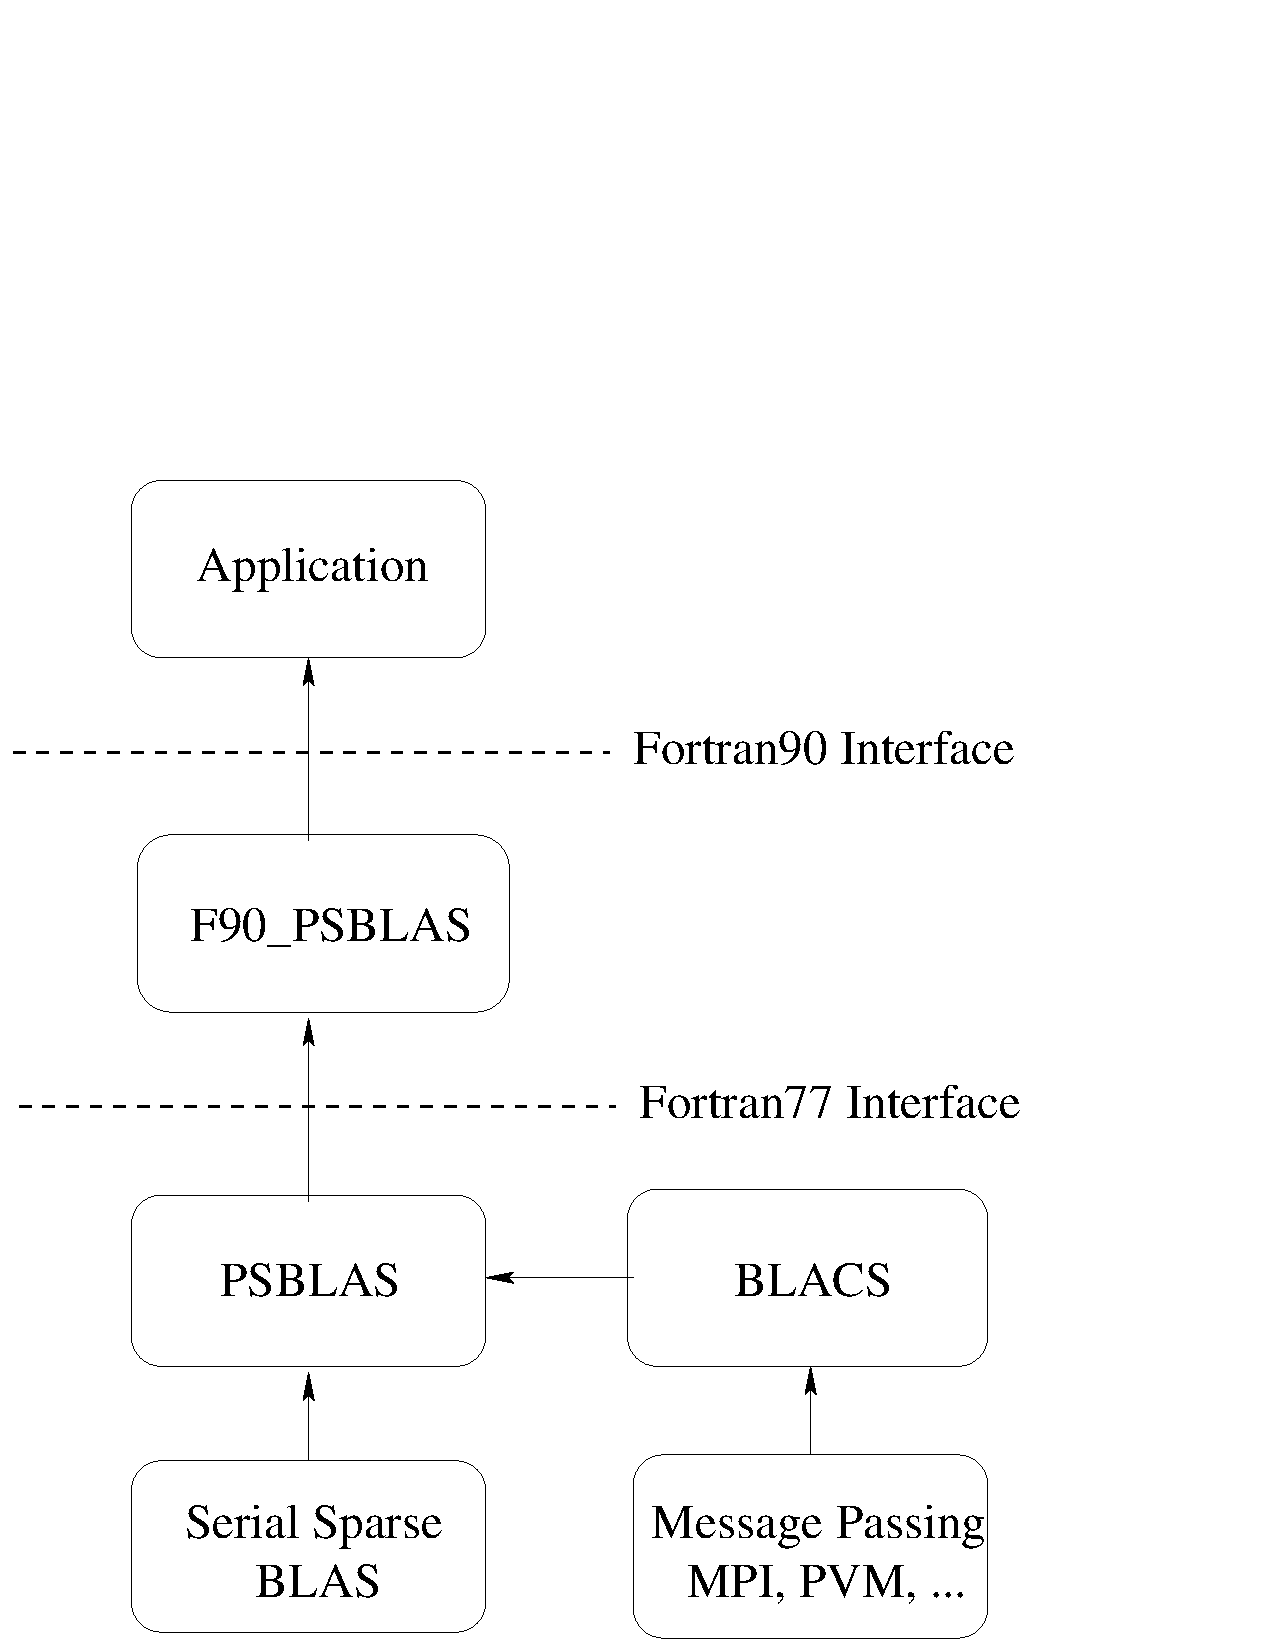
\includegraphics[scale=0.45]{figures/psblas}
\end{center}
\caption{PSBLAS library components hierarchy.\label{fig:psblas}}
\end{figure}

The PSBLAS library consists of two classes of subroutines that is, the
{\em computational routines} and the {\em auxiliary routines}.  The
computational routine set includes:
\begin{itemize}
\item Sparse matrix by dense matrix product; \item Sparse triangular
systems solution for block diagonal matrices;
\item Vector and matrix norms;
\item Dense matrix sums;
\item Dot products.
\end{itemize} 
The auxiliary routine set includes:
\begin{itemize}
\item Communication descriptors allocation;
\item Dense and sparse matrix allocation;
\item Dense and sparse matrix build and update;
\item Sparse matrix and data distribution preprocessing.
\end{itemize} 

The following naming scheme has been adopted for all the symbols
internally defined in the PSBLAS software package:
\begin{itemize}
\item all the symbols (i.e. subroutine names, data types...) are
  prefixed by \verb|psb_| 
\item all the data type names are suffixed by \verb|_type|
\item all the constant values are suffixed by \verb|_|
\item all the subroutine names follow the rule \verb|psb_xxname| where
  \verb|xx| can be either:
  \begin{itemize}
  \item \verb|ge|: the routine is related to dense data, 
  \item \verb|sp|: the routine is related to sparse data, 
  \item \verb|cd|: the routine is related to communication descriptor (see~\ref{sec:datastruct}).
  \end{itemize}
  For example the \verb|psb_geins|, \verb|psb_spins| and
  \verb|psb_cdins| perform the same action (see~\ref{sec:toolsrout}) on
  dense matrices, sparse matrices and communication descriptors
  respectively.
  Interface overloading allows the usage of the same subroutine
  interfaces for both real and complex data.
\end{itemize}
In the description of the subroutines, arguments or argument entries
are classified as:
\begin{description}
\item[global] For input arguments, the value must be the same on all processes
  participating in the subroutine call; for output arguments the value
  is guaranteed to be the same.
\item[local] Each process has its own value(s) independently.
\end{description}

\subsection{Application structure}

The main underlying principle of the PSBLAS library is that the
library objects are created and exist with reference to a discretized
space to which there corresponds an index space and a matrix sparsity
pattern. As an example, consider a cell-centered finite-volume
discretization of  the Navier-Stokes equations on a simulation domain;
the index space $1\dots n$ is isomorphic to the set of cell centers,
whereas the pattern of the associated linear system matrix is
isomorphic to the adjacency graph imposed on the discretization mesh
by the discretization stencil. 

Thus the first order of business is to establish an index space, and
this is done with a call to  \verb|psb_cdall| in which we specify the
size of the index space $n$ and the allocation of the elements of the
index space to the various processes making up the MPI (virtual)
parallel machine. 

The index space is partitioned among processes, and this creates a
mapping from the ``global'' numbering $1\dots n$ to a numbering
``local'' to each process; each process $i$ will own a certain subset
$1\dots n_{\hbox{row}_i}$, each element of which corresponds to a certain
element of $1\dots n$. The user does not set explicitly this mapping;
when the application needs to indicate to which element of the index
space a certain item is related, such as the row and column index of a
matrix coefficient, it does so in the ``global'' numbering, and the
library will translate into the appropriate ``local'' numbering. 

For  a given index space $1\dots n$ there are many possible associated
topologies, i.e. many different discretization stencils; thus the
description of the index space is not completed until the user has
defined a sparsity pattern, either explicitly through \verb|psb_cdins|
or implicitly through \verb|psb_spins|. The descriptor is finalized
with a call to \verb|psb_cdasb| and a sparse matrix with a call to
\verb|psb_spasb|. After \verb|psb_cdasb| each process $i$ will have
defined a set of ``halo'' (or ``ghost'') indices
$n_{\hbox{row}_i}+1\dots n_{\hbox{col}_i}$, denoting elements of the index
space that are \emph{not} assigned to process $i$; however the
variables associated with them are needed to complete computations
associated with the sparse matrix $A$, and thus they have to be
fetched from (neighbouring) processes. The descriptor of the index
space is built exactly for the purpose of properly sequencing the
communication steps required to achieve this objective. 

A simple application structure will walk through the index space
allocation, matrix/vector creation and linear system solution as
follows:
\begin{enumerate}
\item Initialize parallel environment with \verb|blacs_gridinit|
\item Initialize index space with \verb|psb_cdall|
\item Allocate sparse matrix and dense vectors with \verb|psb_spall|
  and \verb|psb_geall|
\item Loop over all local rows, generate matrix and vector entries,
  and insert them with \verb|psb_spins| and \verb|psb_geins|
\item Assemble the various entities: 
\begin{enumerate}
\item \verb|psb_cdasb|
\item \verb|psb_spasb|
\item \verb|psb_geasb|
\end{enumerate}
\item Choose the preconditioner to be used with \verb|psb_precset| and
  build it with \verb|psb_precbld|
\item Call the iterative method of choice, e.g. \verb|psb_bicgstab|
\end{enumerate}
This is the structure of the sample program
\verb|test/pargen/ppde90.f90|. 

For a simulation in which the same discretization mesh is used over
multiple time steps, the following structure may be more appropriate:
\begin{enumerate}
\item Initialize parallel environment with \verb|blacs_gridinit|
\item Initialize index space with \verb|psb_cdall|
\item Loop over the topology of the discretization mesh and build the
  descriptor with \verb|psb_cdins|
\item Assemble the descriptor with \verb|psb_cdasb|
\item Allocate the sparse matrices and dense vectors with
  \verb|psb_spall| and \verb|psb_geall|
\item Loop over the time steps: 
\begin{enumerate}
\item If after first time step, 
  reinitialize the sparse matrix with \verb|psb_sprn|; also zero out
  the dense vectors;
\item Loop over the mesh, generate the coefficients and insert/update
  them with \verb|psb_spins| and \verb|psb_geins|
\item Assemble with \verb|psb_spasb| and \verb|psb_geasb|
\item Choose and build preconditioner with \verb|psb_precset| and
  \verb|psb_precbld|
\item Call the iterative method of choice, e.g. \verb|psb_bicgstab|
 \end{enumerate}
\end{enumerate}
The insertion routines will be called as many times as needed; it is
clear that they only need be called on the data that is actually
allocated to the current process, i.e. each process generates its own
data. 

In principle there is no specific order in the calls to
\verb|psb_spins|, nor is there a requirement to build a matrix row in
its entirety before calling the routine; this allows the application
programmer to walk through the discretization mesh element by element,
generating the main part of a given matrix row but also contributions
to the rows corresponding to neighbouring elements. 

From a functional point of view it is even possible to execute one
call for each nonzero coefficient; however this would have a
substantial computational overhead. It is therefore advisable to pack
a certain amount of data into each call to the insertion routine, say
touching on a few tens of rows; the best performng value would depend
on both the architecture of the computer being used and on the problem
structure. 
At the opposite extreme, it would be possible to generate the entire
part of a coefficient matrix residing on a process and pass it in a
single call to \verb|psb_spins|; this, however, would entail a
doubling of memory occupation, and thus would be almost always far
from optimal. 

\subsection{Programming model}

The PSBLAS librarary is based on the Single Program Multiple Data
(SPMD) programming model: each process participating in the
computation performs the same actions on a chunk of data. Parallelism
is thus data-driven. 

Because of this structure, practically all subroutines \emph{must} be
called simultaneously by all processes participating in the
computation, i.e each subroutine call acts implicitly as a
synchronization point. The exceptions to this rule are:
\begin{itemize}
\item The insertion routines \verb|psb_cdins|, \verb|psb_spins| and
  \verb|psb_geins|;
\item The error handling routines.
\end{itemize}
In particular, as per the discussion in the previous section, the
insertion routines may be called a different number of times on each
process, depending on  the data distribution chosen by the user. 

%%% Local Variables: 
%%% mode: latex
%%% TeX-master: "userguide"
%%% End: 

\section{Data Structures}
\label{sec:datastruct}
%\ifthenelse{\boolean{mtc}}{\minitoc}{}

In this chapter we  illustrate the  data structures used for definition of
routines interfaces. They  include data structures for sparse matrices,
communication descriptors and preconditioners.%%  These data structures
%% are used for calling PSBLAS routines in Fortran~90 language and will
%% be used to next chapters containing these callings.  

All the data types and subroutine interfaces are defined in the module
\verb|psb_sparse_mod|; this will have to be included by every user
subroutine that makes use of the library. 



\subsection{Descriptor data structure}
\label{sec:desc}
All the general matrix informations and elements to be
exchanged among processes are stored within a data structure of the
type \hypertarget{descdata}{{\tt psb\_desc\_type}}. 
Every structure of this type is associated to a sparse matrix, it
contains data about general matrix informations and elements to be
exchanged among processes.  

It is not necessary for the user to know the internal structure of
\verb|psb_desc_type|, it is set in a transparent mode by the tools
routines of Sec.~\ref{sec:toolsrout} while creating a new sparse
matrix; nevertheless we include its description for the curious reader:  
\begin{description}
\item[{\bf matrix\_data}] includes general information about matrix and
process grid. More precisely:
\begin{description}
\item[matrix\_data[psb\_dec\_type\_\hbox{]}] Identifies the decomposition type
(global); the actual values are internally defined, so they should
never be accessed directly.
\item[matrix\_data[psb\_ctxt\_\hbox{]}] Communication context
  associated with the processes comprised in the virtual parallel
  machine (global).
\item[matrix\_data[psb\_m\_\hbox{]}] Total number of equations (global).
\item[matrix\_data[psb\_n\_\hbox{]}] Total number of variables (global).
\item[matrix\_data[psb\_n\_row\_\hbox{]}] Number of grid variables owned by the
current process (local); equivalent to the number of local rows in the
sparse coefficient matrix.
\item[matrix\_data[psb\_n\_col\_\hbox{]}] Total number of grid variables read by the
current process (local); equivalent to the number of local columns in
the sparse coefficient matrix. They include the halo.
\end{description}
Specified as: an allocatable integer array of dimension \verb|psb_mdata_size_|.
\item[{\bf halo\_index}] A list of the halo and boundary elements for
the current process to be exchanged with other processes; for each
processes with which it is necessary to communicate:
\begin{enumerate}
\item Process identifier;
\item Number of points to be received;
\item Indices of points to be received;
\item Number of points to be sent;
\item Indices of points to be sent;
\end{enumerate}
The list may contain an arbitrary number of groups; its end is marked
by a -1.\\
Specified as: an allocatable integer array of rank one.
\item [{\bf ovrlap\_index}] A list of the overlap elements for the
current process, organized in groups like the previous vector:
\begin{enumerate}
\item Process identifier;
\item Number of points to be received;
\item Indices of points to be received;
\item Number of points to be sent;
\item Indices of points to be sent;
\end{enumerate}
The list may contain an arbitrary number of groups; its end is marked
by a -1.\\
Specified as: an allocatable integer array  of rank one.
\item [{\bf ovrlap\_index}] For all overlap points belonging to th
ecurrent process:
\begin{enumerate}
\item  Overlap point index;
\item  Number of processes sharing that overlap points;
\end{enumerate}
The list may contain an arbitrary number of groups; its end is marked
by a -1.\\
Specified as: an allocatable integer array of rank one.
\item[{\bf loc\_to\_glob}] each element $i$ of this array contains
global identifier of the local variable $i$.\\
Specified as: an allocatable integer array of rank one.
\item[{\bf glob\_to\_loc}]  if global variable $i$ is read by current
process then element $i$ contains local index correpondent to global variable $i$;
else element $i$ contains -1 (NULL) value.\\
Specified as: an allocatabled integer array of rank one.
\end{description}
The Fortran95 definition  for \verb|psb_desc_type| structures is 
as follows:
\begin{figure}[h!]
  \begin{Sbox}
    \begin{minipage}[tl]{0.9\textwidth}
\begin{verbatim} 
type psb_desc_type 
   integer, allocatable :: matrix_data(:), halo_index(:)
   integer, allocatable :: overlap_elem(:), overlap_index(:)
   integer, allocatable :: loc_to_glob(:), glob_to_loc(:)
end type psb_desc_type 
\end{verbatim}
    \end{minipage}
  \end{Sbox}
  \setlength{\fboxsep}{8pt}
  \begin{center}
    \fbox{\TheSbox}
  \end{center}
  \caption{\label{fig:desctype}The PSBLAS defined data type that
    contains the communication descriptor.}
\end{figure}

A communication descriptor associated with a sparse  matrix has a
state, which can take the following values:
\begin{description}
\item[Build:] State entered after the first allocation, and before the
  first assembly; in this state it is possible to add communication
  requirements among different processes. 
\item[Assembled:] State entered after the assembly; computations using
  the associated sparse matrix, such as matrix-vector products, are
  only possible   in this state.
\end{description}
\subsubsection{Named Constants}
\label{sec:cd_constants}
\begin{description}
\item[psb\_none\_] Generic no-op;
\item[psb\_nohalo\_]  Do not fetch halo elements;
\item[psb\_halo\_]  Fetch halo elements from neighbouring processes;
\item[psb\_sum\_] Sum overlapped elements
\item[psb\_avg\_] Average overlapped elements
%% \item[psb\_square\_root\_] Update with the square root of the average
%%   of overlapped elements;
\item[psb\_dec\_type\_] Entry holding decomposition type (in \verb|desc_a%matrix_data|)
\item[psb\_m\_] Entry holding total number of rows
\item[psb\_n\_] Entry holding total number of columns
\item[ psb\_n\_row\_] Entry holding the number of rows stored in the
  current process
\item[psb\_n\_col\_] Entry holding the number of columns stored in the
  current process
\item[psb\_ctxt\_] Entry holding a copy of the BLACS communication context
\item[psb\_desc\_asb\_] State of the descriptor: assembled,
      i.e. suitable for computational tasks. 
\item[psb\_desc\_bld\_] State of the descriptor: build, must be
  assembled before computational use.
\end{description}



\subsection{Sparse Matrix data structure}
\label{sec:spmat}
The \hypertarget{spdata}{{\tt psb\_spmat\_type}} data structure
contains all information about local portion of the sparse matrix and   
its storage mode. Most  of these fields are set  by the tools
routines when inserting a new sparse matrix; the user needs only
choose, if he/she so whishes, a specific matrix storage mode. \\
\begin{description}
\item[{\bf aspk}] Contains values of the local distributed sparse
matrix.\\
Specified as: an allocatable array of rank one of type corresponding
to matrix entries type.
\item[{\bf ia1}] Holds integer information on distributed sparse
matrix. Actual information will depend on data format used.\\
Specified as: an allocatable  integer array of rank one.
\item[{\bf ia2}] Holds integer information on distributed sparse
matrix. Actual information will depend on data format used.\\
Specified as: an allocatable  integer array of rank one.
\item[{\bf infoa}] On entry can hold auxiliary information on distributed sparse
matrix.  Actual information will depend on data format used.\\
Specified as: an integer array of length \verb|psb_ifasize_|.
\item[{\bf fida}] Defines the format of the distributed sparse matrix.\\
Specified as: a string of length 5
\item[{\bf descra}] Describe the characteristic of the distributed sparse matrix.\\
Specified as: array of character of length 9.
\item[{\bf pl}] Specifies the local row permutation of distributed sparse
matrix. If pl(1) is equal to 0, then there isn't row permutation.\\
Specified as: an allocatable integer array of dimension equal to number of local row (matrix\_data[psb\_n\_row\_\hbox{]})
\item[{\bf pr}] Specifies the local column permutation of distributed sparse
matrix. If PR(1) is equal to 0, then there isn't columnm permutation.\\
Specified as: an allocatable integer array of dimension equal to number of
local row (matrix\_data[psb\_n\_col\_\hbox{]})
\item[{\bf m}] Number of rows; if row indices are stored explicitly,
as in Coordinate Storage, should be greater than or equal to the
maximum row index actually present in the sparse matrix.
Specified as: integer variable.
\item[{\bf k}] Number of columns; if column indices are stored explicitly,
as in Coordinate Storage or Compressed Sparse Rows, should be greater
than or equal to the maximum column  index actually present in the sparse matrix.
Specified as: integer variable.
\end{description}
FORTRAN95 interface for distributed sparse matrices containing double precision
real entries is defined as in figure~\ref{fig:spmattype}.
\begin{figure}[h!]
  \begin{Sbox}
    \begin{minipage}[tl]{0.85\textwidth}
\begin{verbatim}
type psb_dspmat_type
   integer     :: m, k
   character   :: fida(5)
   character   :: descra(10)
   integer     :: infoa(psb_ifa_size_)
   real(kind(1.d0)), allocatable :: aspk(:)
   integer, allocatable :: ia1(:), ia2(:)
   integer, allocatable :: pr(:), pl(:)
end type psb_dspmat_type
\end{verbatim}
    \end{minipage}
  \end{Sbox}
  \setlength{\fboxsep}{8pt}
  \begin{center}
    \fbox{\TheSbox}
  \end{center}
  \caption{\label{fig:spmattype} 
    The PSBLAS defined data type that
    contains a sparse matrix.} 
\end{figure}

The following two cases are among the most commonly used: 
\begin{description}
\item[fida=``CSR''] Compressed storage by rows. In this case the
following should hold: 
\begin{enumerate}
\item \verb|ia2(i)| contains the index of the first element of row
\verb|i|; the last element of the sparse matrix is thus stored at
index $ia2(m+1)-1$. It should contain \verb|m+1| entries in
nondecreasing order (strictly increasing, if there are no empty rows).
\item \verb|ia1(j)| contains the column index and \verb|aspk(j)|
contains the corresponding coefficient value, for all $ia2(1) \le j
\le ia2(m+1)-1$.
\end{enumerate}
\item[fida=``COO''] Coordinate storage. In this case the following
should hold: 
\begin{enumerate}
\item \verb|infoa(1)| contains the number of nonzero elements in the
matrix; 
\item For all $1 \le j \le infoa(1)$, the coefficient, row index and
column index are stored into \verb|apsk(j)|, \verb|ia1(j)| and
\verb|ia2(j)| respectively. 
\end{enumerate}
\end{description}
A sparse matrix has an associated state, which can take the following
values:
\begin{description}
\item[Build:] State entered after the first allocation, and before the
  first assembly; in this state it is possible to add nonzero entries.
\item[Assembled:] State entered after the assembly; computations using
  the sparse matrix, such as matrix-vector products, are only possible
  in this state;
\item[Update:] State entered after a reinitalization; this is used to
  handle applications in which the same sparsity pattern is used
  multiple times with different coefficients. In this state it is only
  possible to enter coefficients for already existing nonzero entries.
\end{description}
\subsubsection{Named Constants}
\label{sec:sp_constants}
\begin{description}
%% \item[psb\_nztotreq\_] Request to fetch the total number of nonzeroes
%%   stored in a sparse matrix
%% \item[psb\_nzrowreq\_] Request to fetch the number of nonzeroes in a
%%   given row in a sparse matrix
\item[psb\_dupl\_ovwrt\_] Duplicate coefficients should be overwritten
  (i.e. ignore duplications)
\item[psb\_dupl\_add\_] Duplicate coefficients should be added;	         
\item[psb\_dupl\_err\_] Duplicate coefficients should trigger an error conditino
\item[psb\_upd\_dflt\_] Default update strategy for matrix coefficients;
\item[psb\_upd\_srch\_] Update strategy based on search into the data structure;
\item[psb\_upd\_perm\_] Update strategy based on additional
  permutation data (see tools routine description).
\end{description}



\subsection{Preconditioner data structure}
\label{sec:prec}
Our library  offers support for  many different types of
preconditioning schemes. Besides the simple well known preconditioners
like Diagonal Scaling or Block Jacobi with either  incomplete
factorization ILU(0) or complete LU factorization.  We also provide an
experimental package of  complex 
preconditioning methods like the Additive Schwarz and Multilevel
Additive Schwarz; these last preconditioners will be described in a
separate document. 

 A preconditioner is held in the \hypertarget{precdata}{{\tt
    psb\_prec\_type}} data structure which depends on the
\verb|psb_base_prec| reported in 
figure~\ref{fig:prectype}. The \verb|psb_base_prec| 
data type may contain a simple preconditioning matrix with the
associated communication descriptor which may be different than the
system communication descriptor in the case of parallel
preconditioners like the Additive Schwarz one. Then the
\verb|psb_prec_type| may contain more than one preconditioning matrix
like in the case of Two-Level (in general Multi-Level) preconditioners.
The user can choose the type of preconditioner to be used by means of
the \verb|psb_precset| subroutine; once the type of preconditioning
method is specified, along with all the parameters that characterize
it, the preconditioner data structure can be built using the
\verb|psb_precbld| subroutine.
This data structure wants to be flexible enough to easily allow the
implementation of new kind of preconditioners. The values contained in
the \verb|iprcparm| and \verb|dprcparm| define tha type of
preconditioner along with all the parameters related to it; thus,
\verb|iprcparm| and \verb|dprcparm| define how the other records have
to be interpreted.
\begin{figure}[h!]
  \small
  \begin{Sbox}
    \begin{minipage}[tl]{0.9\textwidth}
\begin{verbatim}

  type psb_dbaseprc_type

    type(psb_dspmat_type), allocatable :: av(:) 
    real(kind(1.d0)), allocatable      :: d(:)  
    type(psb_desc_type)                :: desc_data , desc_ac
    integer, allocatable               :: iprcparm(:) 
    real(kind(1.d0)), allocatable      :: dprcparm(:) 
    integer, allocatable               :: perm(:),  invperm(:) 
    integer, allocatable               :: mlia(:), nlaggr(:) 
    type(psb_dspmat_type), pointer     :: base_a    => null() !
    type(psb_desc_type), pointer       :: base_desc => null() ! 
    real(kind(1.d0)), allocatable      :: dorig(:) 

  end type psb_dbaseprc_type
  
  type psb_dprec_type
    type(psb_dbaseprc_type), allocatable  :: baseprecv(:) 
    integer                       :: prec, base_prec
  end type psb_dprec_type

\end{verbatim}
    \end{minipage}
  \end{Sbox}
  \setlength{\fboxsep}{8pt}
  \begin{center}
    \fbox{\TheSbox}
  \end{center}
  \caption{\label{fig:prectype}The PSBLAS defined data type that contains a preconditioner.}
\end{figure}
\subsubsection{Named Constants}
\label{sec:prec_constants}
\begin{description}
\item[f\_ilu\_n\_] Incomplete LU factorization with $n$ levels of
  fill-in; currently only $n=0$ is implemented;
\item[f\_slu\_]  Sparse factorization using SuperLU;
\item[f\_umf\_]  Sparse factorization using UMFPACK;
\item[add\_ml\_prec\_] Additive multilevel correction;
\item[mult\_ml\_prec\_] Multiplicative multilevel correction;
\item[pre\_smooth\_] Pre-smoothing in applying multiplicative
  multilevel corrections;
\item[post\_smooth\_] Post-smoothing in applying multiplicative
  multilevel corrections;
\item[smooth\_both\_] Two-sided (i.e. symmetric) smoothing in applying multiplicative
  multilevel corrections;
\item[mat\_distr\_] Coarse matrix distributed among processes
\item[mat\_repl\_] Coarse matrix replicated among processes
\end{description}


%%% Local Variables: 
%%% mode: latex
%%% TeX-master: "userguide"
%%% End: 

\section{Algebraic routines}

%%%%%%%%%%%%%%%%%%%%%%%%%%%%%%%%%%%%%%%%%%%%%%%%%%
%
%      DENSE MATRIX SUM
%
%%%%%%%%%%%%%%%%%%%%%%%%%%%%%%%%%%%%%%%%%%%%%%%%%%
\subroutine{psb\_geaxpby}{General Dense Matrix Sum}

This subroutine is an interface to the computational kernel for
dense matrix sum:
\[ y \leftarrow  \alpha\> x+ \beta y \] 
where:
\begin{description}
\item[$x$] represents the global dense submatrix $x_{:, jx:jx+n-1}$
\item[$y$] represents the global dense submatrix $y_{:, jy:jy+n-1}$
\end{description}

\syntax{call psb\_geaxpby}{alpha, x, beta, y, desc\_a, info}
\syntax*{call psb\_geaxpby}{alpha, x, beta, y, desc\_a, info, n, jx, jy}

%( calculating y <- alpha*x+beta*y )
\begin{table}[h]
\begin{center}
\begin{tabular}{ll}
\hline
$x$, $y$, $\alpha$, $\beta$ & {\bf Subroutine}\\
\hline
Single Precision Real & psb\_axpby \\
Long Precision Real & psb\_axpby \\
Long Precision Complex & psb\_axpby \\
\hline
\end{tabular}
\end{center}
\caption{Data types\label{tab:f90axpby}}
\end{table}

\begin{description}
\item[\bf On Entry]
\item[alpha] the scalar $\alpha$.\\
Scope: {\bf global} \\
Type: {\bf required} \\
Specified as: a number of the data type indicated in Table~\ref{tab:f90axpby}.
\item[x] the local portion of global dense matrix
$x$.\\
Scope: {\bf local} \\
Type: {\bf required} \\
Specified as: a rank one or two array with the POINTER attribute
containing numbers of type 
specified in Table~\ref{tab:f90axpby}.  The rank of $x$ must be the same of $y$. 
\item[beta] the scalar $\beta$.\\
Scope: {\bf global} \\
Type: {\bf required} \\
Specified as: a number of the data type indicated in Table~\ref{tab:f90axpby}.
\item[y] the local portion of the global dense matrix
$y$. \\
Scope: {\bf local} \\
Type: {\bf required} \\
Specified as:  a rank one or two array with the POINTER
attributecontaining numbers of the type 
indicated in Table~\ref{tab:f90axpby}.  The rank of $y$ must be the same of $x$. 
\item[desc\_a] contains data structures for communications.\\
Scope: {\bf local} \\
Type: {\bf required}\\
Specified as: a structured data of type \descdata.
\item[n] number of columns in dense submatrices $x$ and $y$.\\
Scope: {\bf global} \\
Type: {\bf optional}; can only be present if $x$ and $y$ are of rank 2.\\
Default: \verb|min(size(x,2),size(y,2))|.\\
Specified as: an integer variable $n\ge 0$.
\item[jx]  the column index of the global dense matrix $x$,
identifying the first column of the submatrix $x$.\\
Scope: {\bf global} \\
Type: {\bf optional}; can only be present if $x$ and $y$ are of rank 2.\\
Default: $jx = 1$.\\
Specified as: an integer variable $jx\ge 1$. 
\item[jy]  the column index of the global dense matrix $y$,
identifying the first column of the submatrix $y$.\\
Scope: {\bf global} \\
Type: {\bf optional}; can only be present if $x$ and $y$ are of rank 2.\\
Default: $jy = 1$.\\
Specified as: an integer variable $jy\ge 1$. 

\end{description}

\begin{description}
\item[\bf On Return]
\item[y] the local portion of result submatrix $y$.\\
Scope: {\bf local} \\
Type: {\bf required} \\
Specified as: a rank one or two array containing numbers of the type
indicated in Table~\ref{tab:f90axpby}.
\item[info] the local portion of result submatrix $y$.\\
Scope: {\bf local} \\
Type: {\bf required} \\
An integer value that contains an error code. 
\end{description}


%%%%%%%%%%%%%%%%%%%%%%%%%%%%%%%%%%%%%%%%%%%%%%%%%%
%
%       F90DOT PRODUCT
%
%%%%%%%%%%%%%%%%%%%%%%%%%%%%%%%%%%%%%%%%%%%%%%%%%%

\subroutine{psb\_gedot}{Dot Product}

This function computes dot product between two vectors $x$ and
$y$.\\
If $x$ and $y$ are double precision real or single precision real vectors
computes dot-product as:
\[dot \leftarrow x^T y\]
Else if $x$ and $y$ are double precision complex vectors then computes dot-product as:
\[dot \leftarrow x^H y\]
where:
\begin{description}
\item[$x$] represents the global subvector $x_{:,jx}$
\item[$y$] represents the global subvector $y_{:,jy}$
\end{description}

\syntax{psb\_gedot}{x, y, desc\_a, info}
\syntax*{psb\_gedot}{x, y, desc\_a, info, jx, jy}
\begin{table}[h]
\begin{center}
\begin{tabular}{ll}
\hline
$dot$, $x$, $y$ & {\bf Function}\\
\hline
Single Precision Real & psb\_gedot\\
Long Precision Real & psb\_gedot \\
Long Precision Complex & psb\_gedot \\	
\hline
\end{tabular}
\end{center}
\caption{Data types\label{tab:f90dot}}
\end{table}

\begin{description}
\item[\bf On Entry]
\item[x] the local portion of global dense matrix
$x$. This function computes the location of the first element of
local subarray used, based on $jx$ and the field $matrix\_data$ of $desc\_a$ . \\
Scope: {\bf local} \\
Type: {\bf required} \\
Specified as: a pointer to array of rank one or two
containing numbers of type specified in
Table~\ref{tab:f90dot}. The rank of $x$ must be the same of $y$. 
\item[y] the local portion of global dense matrix
$y$. This function computes the location of the first element of
local subarray used, based on $iy, jy$ and the field $matrix\_data$ of $desc\_a$ . \\
Scope: {\bf local} \\
Type: {\bf required} \\
Specified as: a pointer to array of rank one or two
containing numbers of type specified in
Table~\ref{tab:f90dot}. The rank of $y$ must be the same of $x$. 
\item[desc\_a] contains data structures for communications.\\
Scope: {\bf local} \\
Type: {\bf required}\\
Specified as: a structured data of type \descdata.
\item[jx]  the column index of global dense matrix $x$,
identifying the column of subvector $x$.\\
Scope: {\bf global} \\
Type: {\bf optional}; can only be present if $x$ and $y$ are of rank 2.\\
Default: $jx = 1$.\\

\item[jy]  the column index of global dense matrix $y$,
identifying the column of subvector $y$.\\
Scope: {\bf global} \\
Type: {\bf optional}; can only be present if $x$ and $y$ are of rank 2.\\
Default: $jy = 1$.\\
Specified as: an integer variable $jy\ge 1$. 
\item[\bf On Return] 
\item[Function value] is the dot product of subvectors $x$ and $y$.\\
Scope: {\bf global} \\
Specified as: a number of the data type indicated in Table~\ref{tab:f90dot}.
\item[info] the local portion of result submatrix $y$.\\
Scope: {\bf local} \\
Type: {\bf required} \\
An integer value that contains an error code. 
\end{description}
%%%%%%%%%%%%%%%%%%%%%%%%%%%%%%%%%%%%%%%%%%%%%%%%%%
%
%       F90DOT PRODUCT
%
%%%%%%%%%%%%%%%%%%%%%%%%%%%%%%%%%%%%%%%%%%%%%%%%%%

\subroutine{psb\_gedot}{Generalized Dot Product}

This subroutine computes a series of  dot products among the columns of
two dense matrices  $x$ and $y$: 
\[ res(i) \leftarrow x(:,i)^T y(:,i)\]
If the matrices are complex, then the
usual convention applies, i.e. the conjugate transpose of $x$ is
used. If $x$ and $y$ are of rank one, then $res$ is a scalar, else it
is a rank one array. 

\syntax{psb\_gedot}{res, x, y, desc\_a, info}
\begin{table}[h]
\begin{center}
\begin{tabular}{ll}
\hline
$res$, $x$, $y$ & {\bf Subroutine}\\
\hline
Single Precision Real & psb\_gedot\\
Long Precision Real & psb\_gedot \\
Long Precision Complex & psb\_gedot \\	
\hline
\end{tabular}
\end{center}
\caption{Data types\label{tab:f90mdot}}
\end{table}

\begin{description}
\item[\bf On Entry]
\item[x] the local portion of global dense matrix
$x$. \\
Scope: {\bf local} \\
Type: {\bf required} \\
Specified as: a pointer to array of rank one or two
containing numbers of type specified in
Table~\ref{tab:f90mdot}. The rank of $x$ must be the same of $y$. 
\item[y] the local portion of global dense matrix
$y$. \\
Scope: {\bf local} \\
Type: {\bf required} \\
Specified as: a pointer to array of rank one or two
containing numbers of type specified in
Table~\ref{tab:f90mdot}. The rank of $y$ must be the same of $x$. 
\item[desc\_a] contains data structures for communications.\\
Scope: {\bf local} \\
Type: {\bf required}\\
Specified as: a structured data of type \descdata.
\item[\bf On Return] 
\item[res] is the dot product of subvectors $x$ and $y$.\\
Scope: {\bf global} \\
Specified as: a number or a rank-one array  of the data type indicated
in Table~\ref{tab:f90dot}. 
\item[info] the local portion of result submatrix $y$.\\
Scope: {\bf local} \\
Type: {\bf required} \\
An integer value that contains an error code. 
\end{description}

%%%%%%%%%%%%%%%%%%%%%%%%%%%%%%%%%%%%%%%%%%%%%%%%%%
%
%       VECTOR INFINITY-NORM 
%
%%%%%%%%%%%%%%%%%%%%%%%%%%%%%%%%%%%%%%%%%%%%%%%%%%


\subroutine{psb\_geamax}{Infinity-Norm of Vector}    

This function computes 
 the infinity-norm of a vector $x$.\\
If $x$ is double precision real or single precision real vector
computes infinity norm as:
\[ amax \leftarrow \max_i |x_i|\]
else if $x$ is double precision complex vector then computes infinity-norm  as:
\[ amax \leftarrow \max_i {(|re(x_i)| + |im(x_i)|)}\]
where:
\begin{description}
\item[$x$] represents the global subvector $x_{:,jx}$
\end{description}

\syntax{psb\_geamax}{x, desc\_a, info}
\syntax*{psb\_geamax}{x, desc\_a, info, jx}

\begin{table}[h]
\begin{center}
\begin{tabular}{lll}
\hline
$amax$ & $x$ & {\bf Function}\\
\hline
Single Precision Real&Single Precision Real & psb\_geamax\\
Long Precision Real&Long Precision Real & psb\_geamax \\
Long Precision Real&Long Precision Complex & psb\_zgeamax \\
\hline
\end{tabular}
\end{center}
\caption{Data types\label{tab:f90amax}}
\end{table}


\begin{description}
\item[\bf On Entry]
\item[x] the local portion of global dense matrix
$x$. This function computes the location of the first element of
local subarray used, based on $jx$ and the field $matrix\_data$ of $desc\_a$ . \\
Scope: {\bf local} \\
Type: {\bf required} \\
Specified as:  a rank one or two array with the POINTER attribute 
containing numbers of type specified in
Table~\ref{tab:f90amax}.
\item[desc\_a] contains data structures for communications.\\
Scope: {\bf local} \\
Type: {\bf required}\\
Specified as: a structured data of type \descdata.
\item[jx]  the column index of global dense matrix $x$,
identifying the column of subvector $x$.\\
Scope: {\bf global} \\
Type: {\bf optional}; can only be present if $x$ is of rank 2.\\	
Default: $jx = 1$\\	
Specified as: an integer variable $jx\ge 1$. 

\item[\bf On Return] 
\item[Function value] is the infinity norm of subvector $x$.\\
Scope: {\bf global} \\
Specified as: a number of the data type indicated in Table~\ref{tab:f90amax}.
\item[info] the local portion of result submatrix $y$.\\
Scope: {\bf local} \\
Type: {\bf required} \\
An integer value that contains an error code. 
\end{description}
%%%%%%%%%%%%%%%%%%%%%%%%%%%%%%%%%%%%%%%%%%%%%%%%%%
%
%       Infinity norm
%
%%%%%%%%%%%%%%%%%%%%%%%%%%%%%%%%%%%%%%%%%%%%%%%%%%

\subroutine{psb\_geamax}{Generalized Infinity Norm}

This subroutine computes a series of  infinity norms on the columns of
a  dense matrix  $x$: 
\[ res(i) \leftarrow \max_k |x(k,i)| \]

\syntax{psb\_geamax}{res, x, desc\_a, info}
\begin{table}[h]
\begin{center}
\begin{tabular}{lll}
\hline
$res$&  $x$& {\bf Subroutine}\\
\hline
Single Precision Real  &Single Precision Real  & psb\_geamax\\
Long Precision Real    &Long Precision Real    & psb\_geamax\\
Long Precision Real &Long Precision Complex & psb\_geamax\\	
\hline
\end{tabular}
\end{center}
\caption{Data types\label{tab:f90mamax}}
\end{table}

\begin{description}
\item[\bf On Entry]
\item[x] the local portion of global dense matrix
$x$. \\
Scope: {\bf local} \\
Type: {\bf required} \\
Specified as: a rank one or two array with the POINTER attribute
containing numbers of type specified in
Table~\ref{tab:f90mamax}. 
\item[desc\_a] contains data structures for communications.\\
Scope: {\bf local} \\
Type: {\bf required}\\
Specified as: a structured data of type \descdata.
\item[\bf On Return] 
\item[res] is the infinity norm of the columns of $x$.\\
Scope: {\bf global} \\
Specified as: a number or a rank-one array  of the data type indicated
in Table~\ref{tab:f90amax}. 
\item[info] the local portion of result submatrix $y$.\\
Scope: {\bf local} \\
Type: {\bf required} \\
An integer value that contains an error code. 
\end{description}

%%%%%%%%%%%%%%%%%%%%%%%%%%%%%%%%%%%%%%%%%%%%%%%%%%
%
%       1-NORM OF A VECTOR
%
%%%%%%%%%%%%%%%%%%%%%%%%%%%%%%%%%%%%%%%%%%%%%%%%%%


\subroutine{psb\_geasum}{1-Norm of Vector}    

This function computes the 1-norm of a vector $x$.\\
If $x$ is double precision real or single precision real vector
computes 1-norm as:
\[ asum \leftarrow  \|x_i\|\]
else if $x$ ic double precision complex vector then computes 1-norm  as:
\[ asum \leftarrow \|re(x)\|_1 + \|im(x)\|_1\]
where:
\begin{description}
\item[$x$] represents the global subvector $x_{:,jx}$
\end{description}

\syntax{psb\_geasum}{x, desc\_a, info}
\syntax*{psb\_geasum}{x, desc\_a, info, jx}

\begin{table}[h]
\begin{center}
\begin{tabular}{ll}
\hline
$dot$, $x$, $y$ & {\bf Function}\\
\hline
Single Precision Real & psb\_geasum\\
Long Precision Real & psb\_geasum \\
Long Precision Complex & psb\_geasum \\	
\hline
\end{tabular}
\end{center}
\caption{Data types\label{tab:f90asum}}
\end{table}

\begin{description}
\item[\bf On Entry]
\item[x] the local portion of global dense matrix
$x$. This function computes the location of the first element of 
local subarray used, based on $jx$ and the field $matrix\_data$ of $desc\_a$ . \\
Scope: {\bf local} \\
Type: {\bf required} \\
Specified as: a rank one or two array with the POINTER attribute
containing numbers of type specified in
Table~\ref{tab:f90asum}.
\item[desc\_a] contains data structures for communications.\\
Scope: {\bf local} \\
Type: {\bf required}\\
Specified as: a structured data of type \descdata.
\item[jx]  the column index of global dense matrix $x$,
identifying the column of subvector $x$.\\
Scope: {\bf global} \\
Type: {\bf optional}; can only be present if $x$ is of rank 2.\\	
Default: $jx = 1$\\	
Specified as: an integer variable $jx\ge 1$. 

\item[\bf On Return] 
\item[Function value] is the 1-norm of subvector $x$.\\
Scope: {\bf global} \\
Specified as: a number of the data type indicated in Table~\ref{tab:f90asum}.
\item[info] the local portion of result submatrix $y$.\\
Scope: {\bf local} \\
Type: {\bf required} \\
An integer value that contains an error code. 
\end{description}


%%%%%%%%%%%%%%%%%%%%%%%%%%%%%%%%%%%%%%%%%%%%%%%%%%
%
%       2-NORM OF A VECTOR 
%
%%%%%%%%%%%%%%%%%%%%%%%%%%%%%%%%%%%%%%%%%%%%%%%%%%


\subroutine {psb\_genrm2}{2-Norm of Vector}    

This function computes the 2-norm of a vector $x$.\\
If $x$ is double precision real or single precision real vector
computes 2-norm as:
\[ nrm2 \leftarrow \sqrt{x^T x}\]
else if $x$ is double precision complex vector then computes 2-norm  as:
\[ nrm2 \leftarrow \sqrt{x^H x}\]
where:
\begin{description}
\item[$x$] represents the global subvector $x_{:,jx}$
\end{description}

\begin{table}[h]
\begin{center}
\begin{tabular}{ll}
\hline
$nrm2$, $x$ & {\bf Function}\\
\hline
Single Precision Real & psb\_genrm2\\
Long Precision Real & psb\_genrm2 \\
Long Precision Complex & psb\_genrm2 \\
\hline
\end{tabular}
\end{center}
\caption{Data types\label{tab:f90nrm2}}
\end{table}

\syntax{psb\_genrm2}{x, desc\_a, info}
\syntax*{psb\_genrm2}{x, desc\_a, info, jx}
\begin{description}
\item[\bf On Entry]
\item[x] the local portion of global dense matrix
$x$. This function computes the location of the first element of
local subarray used, based on $jx$ and the field $matrix\_data$ of $desc\_a$ . \\
Scope: {\bf local} \\
Type: {\bf required} \\
Specified as:  a rank one or two array with the POINTER attribute
containing numbers of type specified in
Table~\ref{tab:f90nrm2}.
\item[desc\_a] contains data structures for communications.\\
Scope: {\bf local} \\
Type: {\bf required}\\
Specified as: a structured data of type \descdata.
\item[jx]  the column index of global dense matrix $x$,
identifying the column of subvector $x$.\\
Scope: {\bf global} \\
Type: {\bf optional}; can only be present if $x$ is of rank 2.\\	
Default: $jx = 1$\\	
Specified as: an integer variable $jx\ge 1$. 

\item[\bf On Return] 
\item[Function Value] is the 2-norm of subvector $x$.\\
Scope: {\bf global} \\
Type: {\bf required} \\
Specified as: a number of the data type indicated in Table~\ref{tab:f90nrm2}.
\item[info] the local portion of result submatrix $y$.\\
Scope: {\bf local} \\
Type: {\bf required} \\
An integer value that contains an error code. 
\end{description}

%%%%%%%%%%%%%%%%%%%%%%%%%%%%%%%%%%%%%%%%%%%%%%%%%%
%
%       INFINITY-NORM OF A MATRIX 
%
%%%%%%%%%%%%%%%%%%%%%%%%%%%%%%%%%%%%%%%%%%%%%%%%%%


\subroutine{psb\_spnrmi}{Infinity Norm of Sparse Matrix}    

This function computes the infinity-norm of a matrix $A$:\\

\[ nrmi \leftarrow \|A\|_\infty \]
where:
\begin{description}
\item[$A$] represents the global matrix $A$
\end{description}

\begin{table}[h]
\begin{center}
\begin{tabular}{ll}
\hline
$nrmi$, $A$ & {\bf Function}\\
\hline
Single Precision Real & psb\_spnrmi\\
Long Precision Real & psb\_spnrmi \\
Long Precision Complex & psb\_spnrmi \\
\hline
\end{tabular}
\end{center}
\caption{Data types\label{tab:f90nrmi}}
\end{table}

\syntax{psb\_spnrmi}{A, desc\_a, info}

\begin{description}
\item[\bf On Entry]
\item[a] the local  portion of the global sparse matrix
$A$. \\   
Scope: {\bf local} \\
Type: {\bf required}\\
Specified as: a structured data of type \spdata.
\item[desc\_a] contains data structures for communications.\\
Scope: {\bf local} \\
Type: {\bf required}\\
Specified as: a structured data of type \descdata.
\item[\bf On Return] 
\item[Function value] is the infinity-norm of sparse submatrix $A$.\\
Scope: {\bf global} \\
Specified as: a number of the data type indicated in Table~\ref{tab:f90nrmi}.
\item[info] the local portion of result submatrix $y$.\\
Scope: {\bf local} \\
Type: {\bf required} \\
An integer value that contains an error code. 
\end{description}


%%%%%%%%%%%%%%%%%%%%%%%%%%%%%%%%%%%%%%%%%%%%%%%%%%
%
%       SPARSE MATRIX by DENSE MATRIX PRODUCT
%
%%%%%%%%%%%%%%%%%%%%%%%%%%%%%%%%%%%%%%%%%%%%%%%%%%


\subroutine{psb\_spmm}{Sparse Matrix by Dense Matrix Product}   

This subroutine computes the Sparse Matrix by Dense Matrix Product:

\begin{equation}
y \leftarrow \alpha P_r A P_c x + \beta y
\label{eq:f90spmm_no_tra}
\end{equation}
\begin{equation}
y \leftarrow \alpha P_r A^T P_c x + \beta y
\label{eq:f90spmm_tra}
\end{equation}
\begin{equation}
y \leftarrow \alpha P_r A^H P_c x + \beta y
\label{eq:f90spmm_con}
\end{equation}

where:
\begin{description}
\item[$x$] is the global dense submatrix $x_{:, jx:jx+k-1}$
\item[$y$] is the global dense submatrix $y_{:, jy:jy+k-1}$
\item[$A$] is the global sparse submatrix $A$
\item[$P_r, P_c$] are the permutation matrices.
\end{description}

\begin{table}[h]
\begin{center}
\begin{tabular}{ll}
\hline
$A$, $x$, $y$, $\alpha$, $\beta$ & {\bf Subroutine}\\
\hline
Single Precision Real & psb\_spmm\\
Long Precision Real & psb\_spmm \\
Long Precision Complex & psb\_spmm \\
\hline
\end{tabular}
\end{center}
\caption{Data types\label{tab:f90spmm}}
\end{table}

\syntax{CALL psb\_spmm}{alpha, a, x, beta, y, desc\_a, info}
\syntax*{CALL psb\_spmm}{alpha, a, x, beta, y,desc\_a, info,
trans, k, jx, jy, work} 

\begin{description}
\item[\bf On Entry]
\item[alpha] the scalar $\alpha$.\\
Scope: {\bf global} \\
Type: {\bf required}\\
Specified as: a number of the data type indicated in
Table~\ref{tab:f90spmm}. 
\item[a] the local portion of the sparse matrix
$A$. \\ 
Scope: {\bf local} \\
Type: {\bf required}\\
Specified as: a structured data of type \spdata.
\item[x] the local portion of global dense matrix
$x$. This subroutine computes the location of the first element of
local subarray used, based on $jx$ and the field $matrix\_data$ of $desc\_a$ . \\
Scope: {\bf local} \\
Type: {\bf required} \\
Specified as:  a rank one or two array with the POINTER attribute
containing numbers of type specified in
Table~\ref{tab:f90spmm}.  The rank of $x$ must be the same of $y$. 
\item[beta] the scalar $\beta$.\\
Scope: {\bf global} \\
Type: {\bf required} \\
Specified as: a number of the data type indicated in Table~\ref{tab:f90spmm}.
\item[y] the local portion of global dense matrix
$y$. This subroutine computes the location of the first element of
local subarray used, based on $jy$ and the field $matrix\_data$ of $desc\_a$ . \\
Scope: {\bf local} \\
Type: {\bf required} \\
Specified as:  a rank one or two array with the POINTER attribute
containing numbers of type specified in
Table~\ref{tab:f90spmm}. The rank of $y$ must be the same of $x$. 
\item[desc\_a] contains data structures for communications.\\
Scope: {\bf local} \\
Type: {\bf required}\\
Specified as: a structured data of type \descdata.
\item[trans] indicate what kind of operation to perform.
\begin{description}
\item[trans = N] the operation is specified by equation \ref{eq:f90spmm_no_tra}
\item[trans = T] the operation is specified by equation
\ref{eq:f90spmm_tra}
\item[trans = C] the operation is specified by equation
\ref{eq:f90spmm_con}
\end{description}
Scope: {\bf global} \\
Type: {\bf optional}\\	
Default: $trans = N$\\	
Specified as: a character variable.
\item[k] number of columns in dense submatrices $x$ and $y$. \\
Scope: {\bf global} \\
Type: {\bf optional}\\	
Default: \verb|min(size(x,2)-jx+1,size(y,2)-jy+1)|\\	
Specified as: an integer variable $ k \ge 1$.
\item[jx]  the column index of global dense matrix $x$,
identifying the column of subvector $x$.\\
Scope: {\bf global} \\
Type: {\bf optional}; can only be present if $x$ is of rank 2.\\	
Default: $iy = 1$\\	
Specified as: an integer variable $jx\ge 1$. 
\item[jy]  the column index of global dense matrix $y$,
identifying the column of subvector $y$.\\
Scope: {\bf global} \\
Type: {\bf optional}; can only be present if $y$ is of rank 2.\\	
Default: $jy = 1$\\	
Specified as: an integer variable $jy\ge 1$. 

\item[work] the work array.\\
Scope: {\bf local} \\
Specified as: a rank one array of the same type of $x$ and $y$ with
the POINTER attribute. 

\item[\bf On Return]
\item[y] the local portion of result submatrix $y$.\\
Scope: {\bf local} \\
Type: {\bf required} \\
Specified as: a pointer to array of rank one or two
containing numbers of type specified in
Table~\ref{tab:f90spmm}.
\item[info] the local portion of result submatrix $y$.\\
Scope: {\bf local} \\
Type: {\bf required} \\
An integer value that contains an error code. 
\end{description}

%%%%%%%%%%%%%%%%%%%%%%%%%%%%%%%%%%%%%%%%%%%%%%%%%%
%
%       TRIANGULAR SYSTEM SOLVE
%
%%%%%%%%%%%%%%%%%%%%%%%%%%%%%%%%%%%%%%%%%%%%%%%%%%


\subroutine{psb\_spsm}{Triangular System Solve}   

This subroutine computes the Triangular System Solve:

\begin{eqnarray*}
y &\leftarrow& \alpha P_r T^{-1} P_c x + \beta y\\
y &\leftarrow& \alpha D P_r T^{-1} P_c x + \beta y\\
y &\leftarrow& \alpha P_r T^{-1} P_c D x + \beta y\\
y &\leftarrow& \alpha P_r T^{-T} P_c x + \beta y\\
y &\leftarrow& \alpha D P_r T^{-T} P_c x + \beta y\\
y &\leftarrow& \alpha P_r T^{-T} P_c D x + \beta y\\
y &\leftarrow& \alpha P_r T^{-H} P_c x + \beta y\\
y &\leftarrow& \alpha D P_r T^{-H} P_c x + \beta y\\
y &\leftarrow& \alpha P_r T^{-H} P_c D x + \beta y\\
\end{eqnarray*}


where:
\begin{description}
\item[$x$] is the global dense submatrix $x_{:, jx:jx+n-1}$
\item[$y$] is the global dense submatrix $y_{:, jy:jy+n-1}$
\item[$T$] is the global sparse block triangular submatrix $T$
\item[$D$] is the scaling diagonal matrix.
\item[$P_r, P_c$] are the permutation matrices.
\end{description}

\syntax{CALL psb\_spsm}{alpha, t, x, beta, y, desc\_a, info} 
\syntax*{CALL psb\_spsm}{alpha, t, x, beta, y, desc\_a, info,
trans, unit, choice, diag, n, jx, jy, work} 

\begin{table}[h]
\begin{center}
\begin{tabular}{ll}
\hline
$T$, $x$, $y$, $D$, $\alpha$, $\beta$ & {\bf Subroutine}\\
\hline
Single Precision Real & psb\_spsm\\
Long Precision Real & psb\_spsm \\
Long Precision Complex & psb\_spsm \\
\hline
\end{tabular}
\end{center}
\caption{Data types\label{tab:f90spsm}}
\end{table}



\begin{description}
\item[\bf On Entry]
\item[alpha] the scalar $\alpha$.\\
Scope: {\bf global} \\
Type: {\bf required}\\
Specified as: a number of the data type indicated in
Table~\ref{tab:f90spsm}.
\item[t] the global portion of the sparse matrix
$T$.  \\ 
Scope: {\bf local} \\
Type: {\bf required}\\
Specified as: a structured data type specified in
\S~\ref{sec:datastruct}.
\item[x] the local portion of global dense matrix
$x$. This subroutine computes the location of the first element of
local subarray used, based on $jx$ and the field $matrix\_data$ of $desc\_a$ . \\
Scope: {\bf local} \\
Type: {\bf required} \\
Specified as:  a rank one or two array with the POINTER attribute
containing numbers of type specified in
Table~\ref{tab:f90spsm}.  The rank of $x$ must be the same of $y$. 
\item[beta] the scalar $\beta$.\\
Scope: {\bf global} \\
Type: {\bf required} \\
Specified as: a number of the data type indicated in Table~\ref{tab:f90spsm}.
\item[y] the local portion of global dense matrix
$y$. This subroutine computes the location of the first element of
local subarray used, based on $jy$ and the field $matrix\_data$ of $desc\_a$ . \\
Scope: {\bf local} \\
Type: {\bf required} \\
Specified as:  a rank one or two array with the POINTER attribute
containing numbers of type specified in
Table~\ref{tab:f90spsm}. The rank of $y$ must be the same of $x$. 
\item[desc\_a] contains data structures for communications.\\
Scope: {\bf local} \\
Type: {\bf required}\\
Specified as: a structured data of type \descdata.
\item[trans] specify with {\em unitd} the operation to perform.
\begin{description}
\item[trans = 'N'] the operation is with no transposed matrix
\item[trans = 'T'] the operation is with transposed matrix.
\item[trans = 'C'] the operation is with conjugate transposed matrix.
\end{description}
Scope: {\bf global} \\
Type: {\bf optional}\\	
Default: $trans = N$\\	
Specified as: a character variable.
\item[unitd] specify with {\em trans} the operation to perform.
\begin{description}
\item[unitd = 'U'] the operation is with no scaling
\item[unitd = 'L'] the operation is with left scaling
\item[unitd = 'R'] the operation is with right scaling.
\end{description}
Scope: {\bf global} \\
Type: {\bf optional}\\	
Default: $unitd = U$\\	
Specified as: a character variable.
\item[choice] specify whether a cleanup of the overlapped elements is
required on exit.
\begin{description}
\item[choice = .false.] no cleanup on exit
\item[choice = .true.] cleanup on exit.\\
\end{description}
Scope: {\bf global} \\
Type: {\bf optional}\\	
Default: $choice = .true.$\\	
Specified as: a logical variable.
\item[diag] the diagonal scaling matrix.\\
Scope: {\bf local} \\
Type: {\bf optional}\\	
Default: $diag(1) = 1 (no scaling)$\\	
Specified as: a rank one  array containing numbers of the type
indicated in Table~\ref{tab:f90spsm}.
\item[n] number of columns in dense submatrices $x$ and $y$. \\
Scope: {\bf global} \\
Type: {\bf optional}\\	
Default:  \verb|min(size(x,2)-jx+1,size(y,2)-jy+1)|\\	
Specified as: an integer variable $ n \ge 0$.
\item[jx]  the column index of global dense matrix $x$,
identifying the column of subvector $x$.\\
Scope: {\bf global} \\
Type: {\bf optional}; can only be present if $x$ is of rank 2.\\	
Default: $jx = 1 $\\	
Specified as: an integer variable $jx\ge 1$. 
\item[jy]  the column index of global dense matrix $y$,
identifying the column of subvector $y$.\\
Scope: {\bf global} \\
Type: {\bf optional}; can only be present if $y$ is of rank 2.\\	
Default: $jy = 1 $\\	
Specified as: an integer variable $jy\ge 1$. \\
Scope: {\bf global} \\
Specified as: a number of the data type indicated in Table~\ref{tab:f90spsm}.
\item[work] the work array. \\
Scope: {\bf local} \\
Type: {\bf optional}\\	
Specified as: a rank one array of the same type of $x$ with the
POINTER attribute. 

\item[\bf On Return] 
\item[y] the local portion of global dense matrix
$y$. This subroutine computes the location of the first element of
local subarray used, based on $jy$ and the field $matrix\_data$ of $desc\_a$ . \\
Scope: {\bf local} \\
Type: {\bf required} \\
Specified as: a pointer to array of rank one or two
containing numbers of type specified in
Table~\ref{tab:f90spsm}.
\item[info] the local portion of result submatrix $y$.\\
Scope: {\bf local} \\
Type: {\bf required} \\
An integer value that contains an error code. 
\end{description}




%%% Local Variables: 
%%% mode: latex
%%% TeX-master: "userguide"
%%% End: 

\section{Communication routines}
%%%%%%%%%%%%%%%%%%%%%%%%%%%%%%%%%%%%%%%%%%%%%%%%%%
%
%       HALO DATA COMMUNICATION 
%
%%%%%%%%%%%%%%%%%%%%%%%%%%%%%%%%%%%%%%%%%%%%%%%%%%


\subroutine{psb\_halo}{Halo Data Communication}    

These subroutines restore a consistent status for the halo
elements, and  (optionally) scale the result:

\[ x \leftarrow \alpha x \]
where:
\begin{description}
\item[$x$] is a global dense  submatrix.
\end{description}

\begin{table}[h]
\begin{center}
\begin{tabular}{ll}
\hline
$\alpha$, $x$ & {\bf Subroutine}\\
\hline
Single Precision Real & psb\_halo\\
Long Precision Real & psb\_halo \\
Long Precision Complex & psb\_halo \\
\hline
\end{tabular}
\end{center}
\caption{Data types\label{tab:f90halo}}
\end{table}

\syntax{CALL psb\_halo}{x, desc\_a, info}
\syntax*{CALL psb\_halo}{x, desc\_a, info, alpha, work}

\begin{description}
\item[\bf On Entry]
\item[x] global dense matrix $x$.\\
Scope: {\bf local} \\
Type: {\bf required} \\
Specified as:  a rank one or two array with the POINTER attribute
containing numbers of type specified in
Table~\ref{tab:f90halo}.
\item[desc\_a] contains data structures for communications.\\
Scope: {\bf local} \\
Type: {\bf required}\\
Specified as: a structured data type specified in
\S~\ref{sec:datastruct}.
\item[alpha] the scalar $\alpha$.\\
Scope: {\bf global} \\
Type: {\bf optional} \\
Default: $alpha = 1 $\\	
Specified as: a number of the data type indicated in Table~\ref{tab:f90halo}.
\item[work] the work array. \\
Scope: {\bf local} \\
Type: {\bf optional}\\
Specified as: a rank one array of the same type of $x$ with the
POINTER attribute.

\item[\bf On Return] 
\item[x] global dense result matrix $x$.\\
Scope: {\bf local} \\
Type: {\bf required} \\
Returned as:  a rank one or two array with the POINTER attribute
containing numbers of type specified in
Table~\ref{tab:f90halo}.
\item[info] the local portion of result submatrix $y$.\\
Scope: {\bf local} \\
Type: {\bf required} \\
An integer value that contains an error code. 
\end{description}
%%%%%%%%%%%%%%%%%%%%%%%%%%%%%%%%%%%%%%%%%%%%%%%%%%
%
%       OVERLAP UPDATE
%
%%%%%%%%%%%%%%%%%%%%%%%%%%%%%%%%%%%%%%%%%%%%%%%%%%


\subroutine{psb\_ovrl}{Overlap Update}    

These subroutines restore a consistent status for the overlap
elements:

\[ x \leftarrow Q x \]
where:
\begin{description}
\item[$x$] is the global dense submatrix $x$
\item[$Q$] is the overlap operator; it is the composition of two
operators $ P_a$ and $ P^{T}$. 
\end{description}

\begin{table}[h]
\begin{center}
\begin{tabular}{ll}
\hline
$x$ & {\bf Subroutine}\\
\hline
Single Precision Real & psb\_ovrl\\
Long Precision Real & psb\_ovrl \\
Long Precision Complex & psb\_ovrl \\
\hline
\end{tabular}
\end{center}
\caption{Data types\label{tab:f90ovrl}}
\end{table}

\syntax{CALL psb\_ovrl}{x, desc\_a, info}
\syntax*{CALL psb\_ovrl}{x, desc\_a, info, choice=choice,
update\_type=update\_type, work=work} 

\begin{description}
\item[\bf On Entry]
\item[x] global dense matrix $x$.\\
Scope: {\bf local} \\
Type: {\bf required} \\
Specified as:  a rank one or two array with the POINTER attribute
containing numbers of type specified in
Table~\ref{tab:f90ovrl}.
\item[desc\_a] contains data structures for communications.\\
Scope: {\bf local} \\
Type: {\bf required}\\
Specified as: a structured data type specified in
\S~\ref{sec:datastruct}.
item[choice] specify if exchange overlap elements.
\begin{description}
\item[choice = .true.] exchange overlap elements, i.e. apply operator
$P^{T}$;
\item[choice = .false.] don't exchange overlap elements
\end{description}
Scope: {\bf global} \\
Type: {\bf optional} \\
Default: $choice = .true. $\\	
Specified as: a logical variable.
\begin{description}
\item[update\_type = 1] normal update $P_a$;
\item[update\_type = 2] square root update $\sqrt{P_a}$;
\end{description}
Scope: {\bf global} \\
Default: $update\_type = .true. $\\	
Scope: {\bf global} \\
Specified as: a integer variable.
\item[work] the work array. \\
Scope: {\bf local} \\
Type: {\bf optional}\\
Specified as: a one dimensional array of the same type of $x$.

\item[\bf On Return] 
\item[x] global dense result matrix $x$.\\
Scope: {\bf local} \\
Type: {\bf required} \\
Specified as: a pointer to array of rank one or two
containing numbers of type specified in
Table~\ref{tab:f90ovrl}.
\item[info] the local portion of result submatrix $y$.\\
Scope: {\bf local} \\
Type: {\bf required} \\
An integer value that contains an error code. 
\end{description}


\section*{Usage notes}
\begin{enumerate}
\item If there is no overlap in the data distribution, no operations
are performed;
\item The operator $P^{T}$ performs the reduction sum of overlap
elements; it is the inverse of a ``stretch'' operator $P$ that
replicates overlap elements, accounting for the physical replication
of data;
\item The operator $P_a$ performs a scaling on the overlap elements by
the amount of replication; thus, when combined with the reduction
operator, it implements the average of replicated elements over all of
their instances. 
\item The square root update option makes it possible to applythe
following operator: 
\[ x\leftarrow \sqrt{P_a} P^{T} K^{-1} P \sqrt{P_a} x\]
In the case of a symmetric $K$, this preserves simmetry of the overall
preconditioner, which would otherwise be destroyed. 
\end{enumerate}


%%%%%%%%%%%%%%%%%%%%%%%%%%%%%%%%%%%%%%%%%%%%%%%%%%
%
%      GATHER GLOBAL DENSE MATRIX
%
%%%%%%%%%%%%%%%%%%%%%%%%%%%%%%%%%%%%%%%%%%%%%%%%%%

\subroutine{psb\_gather}{Gather Global Dense Matrix}

These subroutines collect the portions of global dense matrix
distributed over all process into one single array stored on one
process.

\[ glob\_x \leftarrow collect(loc\_x_i) \]
where:
\begin{description}
\item[$glob\_x$] is the global submatrix $glob\_x_{iy:iy+m-1,jy:jy+n-1}$
\item[$loc\_x_i$] is the local portion of global dense matrix on
process $i$.
\item[$collect$] is the collect function.
\end{description}

\begin{table}[h]
\begin{center}
\begin{tabular}{ll}
\hline
$x_i, y$ & {\bf Subroutine}\\
\hline
Single Precision Real & psb\_gather\\
Long Precision Real & psb\_gather \\
Long Precision Complex & psb\_gather \\
\hline
\end{tabular}
\end{center}
\caption{Data types\label{tab:gather}}
\end{table}

\syntax{call psb\_gather}{glob\_x, loc\_x, desc\_a, info, 
  root, iglobx, jglobx, ilocx, jlocx, k}
\syntax{call psb\_gather}{glob\_x, loc\_x, desc\_a, info, 
  root, iglobx, ilocx}

\begin{description}
\item[\bf On Entry]
\item[loc\_x] the local portion of global dense matrix
$glob\_x$. \\
Scope: {\bf local} \\
Type: {\bf required}\\
Specified as: a rank one or two array containing numbers of the type
indicated in Table~\ref{tab:gather}.
\item[desc\_a] contains data structures for communications.\\
Scope: {\bf local} \\
Type: {\bf required}\\
Specified as: a structured data type specified in \S~\ref{sec:datastruct}.
\item[root]  The process that holds the global copy. If $root=-1$ all
  the processes will have a copy of the global vector.\\
Scope: {\bf global} \\
Type: {\bf optional}\\
Specified as: an integer variable $0\le ix\le np$. 
\item[iglobx]  Row index to define a submatrix in glob\_x into which
  gather the local pieces.\\
Scope: {\bf global} \\
Type: {\bf optional}\\
Specified as: an integer variable $1\le ix\le matrix\_data(psb\_m\_)$. 
\item[jglobx]  Column index to define a submatrix in glob\_x into which
  gather the local pieces.\\
Scope: {\bf global} \\
Type: {\bf optional}\\
Specified as: an integer variable. 
\item[ilocx]  Row index to define a submatrix in loc\_x that has to
  be gathered into glob\_x.\\
Scope: {\bf local} \\
Type: {\bf optional}\\
Specified as: an integer variable. 
\item[jlocx]  Columns index to define a submatrix in loc\_x that has
  to be gathered into glob\_x.\\
Scope: {\bf global} \\
Type: {\bf optional}\\
Specified as: an integer variable.
\item[k]  The number of columns to gather.\\
Scope: {\bf global} \\
Type: {\bf optional}\\
Specified as: an integer variable. 
\item[\bf On Return] 
\item[glob\_x] The array where the local parts must be gathered.\\
Scope: {\bf global} \\
Type: {\bf required}\\
Specified as: a rank one or two array.
\item[info] the local portion of result submatrix $y$.\\
Scope: {\bf local} \\
Type: {\bf required} \\
An integer value that contains an error code. 
\end{description}

%%%%%%%%%%%%%%%%%%%%%%%%%%%%%%%%%%%%%%%%%%%%%%%%%%
%
%      SCATTER GLOBAL DENSE MATRIX
%
%%%%%%%%%%%%%%%%%%%%%%%%%%%%%%%%%%%%%%%%%%%%%%%%%%

\subroutine{psb\_scatter}{Scatter Global Dense Matrix}

These subroutines scatters the portions of global dense matrix owned
by a process to all the processes in the processes grid.

\[ loc\_x_i \leftarrow scatter(glob\_x_i) \]
where:
\begin{description}
\item[$glob\_x$] is the global submatrix $glob\_x_{iy:iy+m-1,jy:jy+n-1}$
\item[$loc\_x_i$] is the local portion of global dense matrix on
process $i$.
\item[$scatter$] is the scatter function.
\end{description}

\begin{table}[h]
\begin{center}
\begin{tabular}{ll}
\hline
$x_i, y$ & {\bf Subroutine}\\
\hline
Single Precision Real & psb\_scatter\\
Long Precision Real & psb\_scatter \\
Long Precision Complex & psb\_scatter \\
\hline
\end{tabular}
\end{center}
\caption{Data types\label{tab:scatter}}
\end{table}

\syntax{call psb\_scatter}{glob\_x, loc\_x, desc\_a, info, 
  root, iglobx, jglobx, ilocx, jlocx, k}
\syntax{call psb\_scatter}{glob\_x, loc\_x, desc\_a, info, 
  root, iglobx, ilocx}

\begin{description}
\item[\bf On Entry]
\item[glob\_x] The array that must be scattered into local pieces.\\
Scope: {\bf global} \\
Type: {\bf required}\\
Specified as: a rank one or two array.
\item[desc\_a] contains data structures for communications.\\
Scope: {\bf local} \\
Type: {\bf required}\\
Specified as: a structured data type specified in \S~\ref{sec:datastruct}.
\item[root]  The process that holds the global copy. If $root=-1$ all
  the processes have a copy of the global vector.\\
Scope: {\bf global} \\
Type: {\bf optional}\\
Specified as: an integer variable $0\le ix\le np$. 
\item[iglobx]  Row index to define a submatrix in glob\_x that has to
  be scattered into local pieces.\\
Scope: {\bf global} \\
Type: {\bf optional}\\
Specified as: an integer variable $1\le ix\le matrix\_data(psb\_m\_)$. 
\item[jglobx]  Column index to define a submatrix in glob\_x that has to
  be scattered into local pieces.\\
Scope: {\bf global} \\
Type: {\bf optional}\\
Specified as: an integer variable. 
\item[ilocx]  Row index to define a submatrix in loc\_x into which
  scatter the local piece of glob\_x.\\
Scope: {\bf local} \\
Type: {\bf optional}\\
Specified as: an integer variable. 
\item[jlocx]  Columns index to define a submatrix in loc\_x into which
  scatter the local piece of glob\_x.\\
Scope: {\bf global} \\
Type: {\bf optional}\\
Specified as: an integer variable.
\item[k]  The number of columns to scatter.\\
Scope: {\bf global} \\
Type: {\bf optional}\\
Specified as: an integer variable. 
\item[\bf On Return] 
\item[loc\_x] the local portion of global dense matrix
$glob\_x$. \\
Scope: {\bf local} \\
Type: {\bf required}\\
Specified as: a rank one or two array containing numbers of the type
indicated in Table~\ref{tab:scatter}.
\item[info] the local portion of result submatrix $y$.\\
Scope: {\bf local} \\
Type: {\bf required} \\
An integer value that contains an error code. 
\end{description}

%%% Local Variables: 
%%% mode: latex
%%% TeX-master: "userguide"
%%% End: 

\section{Data management routines}
\label{sec:toolsrout}


%
%%   psb_cdall %%
%
\subroutine{psb\_cdall}{Allocates a communication descriptor}

\syntax{call psb\_cdall}{icontxt, desc\_a, info,mg=mg,parts=parts}
\syntax*{call psb\_cdall}{icontxt, desc\_a, info,vg=vg,flag=flag}
\syntax*{call psb\_cdall}{icontxt, desc\_a, info,vl=vl}

This subroutine initializes the communication descriptor associated
with an index space. Exactly one of the  optional arguments
\verb|parts|, \verb|vg|, \verb|vl| must be specified, thereby choosing
the specific initialization strategy:
\begin{description}
\item[\bf  On Entry ]
\item[icontxt] the communication context.\\
Scope:{\bf global}.\\
Type:{\bf required}.\\
Specified as: an integer value.
\item[vg] Data allocation: each index $i\in \{1\dots mg\}$ is allocated
  to process $vg(i)$.
Scope:{\bf global}.\\
Type:{\bf optional}.\\
Specified as: an integer array. 
\item[flag] Specifies whether entries in $vg$ are zero- or one-based.
Scope:{\bf global}.\\
Type:{\bf optional}.\\
Specified as: an integer value $0,1$, default $0$.

\item[mg] the (global) number of rows of the problem.\\
Scope:{\bf global}.\\
Type:{\bf optional}.\\
Specified as: an integer value. It is required if \verb|parts| is
specified. 
\item[parts] the subroutine that defines the partitioning scheme.\\
Scope:{\bf global}.\\
Type:{\bf required}.\\
Specified as: a subroutine. 
\item[vl] Data allocation: the set of global indices belonging to the
  calling process. 
Scope:{\bf local}.\\
Type:{\bf optional}.\\
Specified as: an integer array. 
\end{description}

\begin{description}
\item[\bf On Return]
\item[desc\_a] the communication descriptor.\\
Scope:{\bf local}.\\
Type:{\bf required}.\\
Specified as: a structured data of type \descdata.
\item[info] Error code.\\
Scope: {\bf local} \\
Type: {\bf required} \\
An integer value; 0 means no error has been detected. 
\end{description}

\section*{Notes}
\begin{enumerate}
\item Exactly one of the optional arguments  \verb|parts|, \verb|vg|,
  \verb|vl| must be specified, thereby choosing the initialization
  strategy as follows:
\begin{description}
\item[parts] In this case we have a subroutine specifying the mapping
  between global indices and process/local index pairs. If this
  optional argument   is specified, then it is mandatory to 
  specify the argument \verb|mg| as well.  
  The subroutine must conform to the following interface: 
\begin{verbatim}
  interface 
     subroutine psb_parts(glob_index,mg,np,pv,nv)
       integer, intent (in)  :: glob_index,np,mg
       integer, intent (out) :: nv, pv(*)
     end subroutine psb_parts
  end interface
\end{verbatim}
  The input arguments are:
  \begin{description}
    \item[glob\_index] The global index to be mapped;
    \item[np] The number of processes in the mapping;
    \item[mg] The total number of global rows in the mapping;
  \end{description}
  The output arguments are:
  \begin{description}
    \item[nv] The number of entries in \verb|pv|;
    \item[pv] A vector containint the indices of the processes to
    which the global index should be assigend; each entry must satisfy
    $0\le pv(i) < np$; if $nv>1$ we have an index assigned to multiple
    processes, i.e. we have an overlap among the subdomains.
  \end{description}
\item[vg] In this case the association between an index and a process
  is specified via an integer vector; the size of the index space is
  equal to the size of \verb|vg|, and each index $i$ is assigned to
  the process $vg(i)$. The vector \verb|vg| must be identical on all
  calling processes; its entries may have the ranges $(0\dots np-1)$
  or $(1\dots np)$ according to the value of \verb|flag|.
\item[vl] In this case we are specifying the list of indices assigned
  to the current process; thus, the global problem size $mg$ is given by
  the sum of the sizes of the individual vectors \verb|vl| specified
  on the calling processes. The subroutine will check that each entry
  in the global index space $(1\dots mg)$ is specified exactly once. 
\end{description}
\item On exit from this routine the descriptor is in the build state
\end{enumerate}


%
%%   psb_cdins %%
%
\subroutine{psb\_cdins}{Communication descriptor insert routine}

\syntax{call psb\_cdins}{nz, ia, ja, desc\_a, info}

\begin{description}
\item[\bf On Entry]
\item[nz] the number of points being inserted.\\
Scope: {\bf local}.\\
Type: {\bf required}.\\
Specified as: an integer value.
\item[ia] the row indices of the points being inserted.\\
Scope: {\bf local}.\\
Type: {\bf required}.\\
Specified as: an integer array of length $nz$.
\item[ja] the column indices of the points being inserted.\\
Scope: {\bf local}.\\
Type: {\bf required}.\\
Specified as: an integer array of length $nz$.
%% \item[is] the row offset.\\
%% Scope:{\bf local}.\\
%% Type:{\bf optional}.\\
%% Specified as: an integer value.
%% \item[js] the column offset.\\
%% Scope: {\bf local}.\\
%% Type: {\bf optional}.\\
%% Specified as: an integer value.
\end{description}

\begin{description}
\item[\bf On Return]
\item[desc\_a] the updated communication descriptor.\\
Scope:{\bf local}.\\
Type:{\bf required}.\\
Specified as: a structured data of type \descdata.
\item[info] Error code.\\
Scope: {\bf local} \\
Type: {\bf required} \\
An integer value; 0 means no error has been detected. 
\end{description}
\section*{Notes}
\begin{enumerate}
\item This routine may only be called if the descriptor is in the
  build state
\end{enumerate}



%
%%   psb_cdasb %%
%
\subroutine{psb\_cdasb}{Communication descriptor assembly routine}

\syntax{call psb\_cdasb}{desc\_a, info}

\begin{description}
\item[\bf On Entry]
\item[desc\_a] the communication descriptor.\\
Scope:{\bf local}.\\
Type:{\bf required}.\\
Specified as: a structured data of type \descdata.
\end{description}

\begin{description}
\item[\bf On Return]
\item[info] Error code.\\
Scope: {\bf local} \\
Type: {\bf required} \\
An integer value; 0 means no error has been detected. 
%\item[arg] 
\end{description}
\section*{Notes}
\begin{enumerate}
\item On exit from this routine the descriptor is in the assembled
  state. 
\end{enumerate}



%
%%   psb_cdcpy %%
%
\subroutine{psb\_cdcpy}{Copies a communication descriptor}

\syntax{call psb\_cdcpy}{desc\_out, desc\_a, info}

\begin{description}
\item[\bf On Entry]
\item[desc\_a] the communication descriptor.\\
Scope:{\bf local}.\\
Type:{\bf required}.\\
Specified as: a structured data of type \descdata.

\end{description}

\begin{description}
\item[\bf On Return]
\item[desc\_out] the communication descriptor copy.\\
Scope:{\bf local}.\\
Type:{\bf required}.\\
Specified as: a structured data of type \descdata.
\item[info] Error code.\\
Scope: {\bf local} \\
Type: {\bf required} \\
An integer value; 0 means no error has been detected. 
\end{description}


%
%%   psb_cdfree %%
%
\subroutine{psb\_cdfree}{Frees a communication descriptor}

\syntax{call psb\_cdfree}{desc\_a, info}

\begin{description}
\item[\bf On Entry]
\item[desc\_a] the communication descriptor to be freed.\\
Scope:{\bf local}.\\
Type:{\bf required}.\\
Specified as: a structured data of type \descdata.
\end{description}

\begin{description}
\item[\bf On Return]
\item[info] Error code.\\
Scope: {\bf local} \\
Type: {\bf required} \\
An integer value; 0 means no error has been detected. 
\end{description}



%
%%   psb_cdcpy %%
%
\subroutine{psb\_cdbldext}{Build an extended  communication descriptor}

\syntax{call psb\_cdbldext}{a,desc\_a,nl,desc\_out, info, extype}

This subroutine builds an extended communication descriptor, based on
the input descriptor \verb|desc_a| and on the stencil specified
through the input sparse matrix \verb|a|. 
\begin{description}
\item[\bf On Entry]
\item[a] A sparse matrix
Scope:{\bf local}.\\
Type:{\bf required}.\\
Specified as: a structured data type.
\item[desc\_a] the communication descriptor.\\
Scope:{\bf local}.\\
Type:{\bf required}.\\
Specified as: a structured data of type \spdata.
\item[nl] the number of layers desired.\\
Scope:{\bf global}.\\
Type:{\bf required}.\\
Specified as: an integer value $nl\ge 0$. 
\item[extype] the kind of estension required.\\
Scope:{\bf global}.\\
Type:{\bf optional }.\\
Specified as: an integer value
\verb|psb_ovt_xhal_|, \verb|psb_ovt_asov_|, default: \verb|psb_ovt_xhal_|

\end{description}

\begin{description}
\item[\bf On Return]
\item[desc\_out] the extended communication descriptor.\\
Scope:{\bf local}.\\
Type:{\bf required}.\\
Specified as: a structured data of type \descdata.
\item[info] Error code.\\
Scope: {\bf local} \\
Type: {\bf required} \\
An integer value; 0 means no error has been detected. 
\end{description}


%% %
%% %%   psb_cdren %%
%% %
%% \subroutine{psb\_cdren}{Applies a renumeration to a communication descriptor}

%% \syntax{call psb\_cdren}{trans, iperm, desc\_a, info}

%% \begin{description}
%% \item[\bf On Entry]
%% \item[trans] A character that specifies whether to permute $A$  or $A^T$.\\
%% Scope: {\bf local} \\
%% Type: {\bf required}\\
%% Specified as: a single character with value 'N' for $A$ or 'T' for $A^T$.\\
%% \item[iperm] An integer array containing permutation information.\\
%% Scope: {\bf local} \\
%% Type: {\bf required}\\
%% Specified as: an integer one-dimensional array.\\
%% \item[desc\_a] the communication descriptor.\\
%% Scope:{\bf local}.\\
%% Type:{\bf required}.\\
%% Specified as: a structured data of type \descdata.
%% \end{description}

%% \begin{description}
%% \item[\bf On Return]
%% \item[info] Error code.
%% Scope: {\bf local} \\
%% Type: {\bf required}\\
%% Specified as: an integer variable.
%% \end{description}




%
%%   psb_descprt %%
%
%% \subroutine{psb\_cdprt}{Prints a descriptor}

%% \syntax{call psb\_cdprt}{iout, desc\_a, glob, short}

%% \begin{description}
%% \item[\bf On Entry]
%% \item[iout] An integer that defines the output unit.
%% Scope: {\bf local} \\
%% Type: {\bf required}\\
%% Specified as: Integer scalar.\\
%% \item[desc\_a] The communication descriptor of type \descdata that
%%   must be printed.\\
%% Scope: {\bf local} \\
%% Type: {\bf required}\\
%% Specified as: a variable of type \descdata.\\
%% \end{description}

%% \begin{description}
%% \item[\bf On Return]
%% \item[glob] ??????
%% \item[short] ??????
%% \end{description}



%
%%   psb_spalloc %%
%
\subroutine{psb\_spall}{Allocates a sparse matrix}

\syntax{call psb\_spall}{a, desc\_a, info, nnz}

\begin{description}
\item[\bf On Entry]
\item[desc\_a] the communication descriptor.\\
Scope:{\bf local}.\\
Type:{\bf required}.\\
Specified as: a structured data of type \descdata.
\item[nnz] An estimate of the number of nonzeroes in the local
  part of the assembled matrix.\\ 
Scope: {\bf global}.\\
Type: {\bf optional}.\\
Specified as: an integer value. 
\end{description}

\begin{description}
\item[\bf On Return]
\item[a] the matrix to be allocated.\\
Scope:{\bf local}\\
Type:{\bf required}\\
Specified as: a structured data of type \spdata.
\item[info] Error code.\\
Scope: {\bf local} \\
Type: {\bf required} \\
An integer value; 0 means no error has been detected. 
\end{description}
\section*{Notes}
\begin{enumerate}
\item On exit from this routine the sparse matrix  is in the build
  state.
\item The descriptor may be in either the build or assembled state.
\item Providing a good estimate for the number of nonzeroes $nnz$ in
  the assembled matrix may substantially improve performance in the
  matrix build phase, as it will reduce or eliminate the need for
  (potentially multiple) data reallocations. 
\end{enumerate}



%
%%   psb_spins %%
%
\subroutine{psb\_spins}{Insert a cloud of elements into a sparse matrix}

\syntax{call psb\_spins}{nz, ia, ja, val, a, desc\_a, info}

\begin{description}
\item[\bf On Entry]
\item[nz] the number of elements to be inserted.\\
Scope:{\bf local}.\\
Type:{\bf required}.\\
Specified as: an integer scalar.
\item[ia] the row indices of the elements to be inserted.\\
Scope:{\bf local}.\\
Type:{\bf required}.\\
Specified as: an integer array of size $nz$.
\item[ja] the column indices of the elements to be inserted.\\
Scope:{\bf local}.\\
Type:{\bf required}.\\
Specified as: an integer array of size $nz$.
\item[val] the elements to be inserted.\\
Scope:{\bf local}.\\
Type:{\bf required}.\\
Specified as: an array of size $nz$.
\item[desc\_a] The communication descriptor.\\
Scope: {\bf local}. \\
Type: {\bf required}.\\
Specified as: a variable of type \descdata.\\
%% \item[is] the starting row on matrix $a$.\\
%% Scope:{\bf local}.\\
%% Type:{\bf optional}.\\
%% Specified as: an integer vaule.
%% \item[js] the starting column on matrix $a$.\\
%% Scope:{\bf local}.\\
%% Type:{\bf optional}\\
%% Specified as: an integer value
\end{description}

\begin{description}
\item[\bf On Return]
\item[a] the matrix into which elements will be inserted.\\
Scope:{\bf local}\\
Type:{\bf required}\\
Specified as: a structured data of type \spdata.
\item[desc\_a] The communication descriptor.\\
Scope: {\bf local}. \\
Type: {\bf required}.\\
Specified as: a variable of type \descdata.\\
\item[info] Error code.\\
Scope: {\bf local} \\
Type: {\bf required} \\
An integer value; 0 means no error has been detected. 
\end{description}

\section*{Notes}
\begin{enumerate}
\item On entry to this routine the descriptor may be in either the
  build or assembled state.
\item On entry to this routine the sparse matrix may be in either the
  build or update state. 
\item If the descriptor is in the build state, then the sparse matrix
  must also be in the build state; the action of the routine is to
  (implicitly) call \verb|psb_cdins| to add entries to the sparsity
  pattern;
\item If the descriptor is in the assembled state, then any entries in
  the sparse matrix that would generate additional communication
  requirements will be ignored; 
\item If the matrix is in the update state, any entries in positions
  that were not present in the original matrix will be ignored. 
\end{enumerate}

%
%%   psb_spasb %%
%
\subroutine{psb\_spasb}{Sparse matrix assembly routine}

\syntax{call psb\_spasb}{a, desc\_a, info, afmt, upd, dupl}

\begin{description}
\item[\bf On Entry]
\item[desc\_a] the communication descriptor.\\
Scope:{\bf local}.\\
Type:{\bf required}.\\
Specified as: a structured data of type \descdata.
\item[afmt] the storage format for the sparse matrix.\\
Scope: {\bf global}.\\
Type: {\bf optional}.\\
Specified as: an array of characters. Defalt:  'CSR'.
\item[upd] Provide for updates to the matrix coefficients.\\
Scope: {\bf global}.\\
Type: {\bf optional}.\\
Specified as: integer, possible values: \verb|psb_upd_srch_|, \verb|psb_upd_perm_|
\item[dupl] How to handle duplicate coefficients.\\
Scope: {\bf global}.\\
Type: {\bf optional}.\\
Specified as: integer, possible values: \verb|psb_dupl_ovwrt_|,
\verb|psb_dupl_add_|, \verb|psb_dupl_err_|.
\end{description}

\begin{description}
\item[\bf On Return]
\item[a] the matrix to be assembled.\\
Scope:{\bf local}\\
Type:{\bf required}\\
Specified as: a structured data of type \spdata.
\item[info] Error code.\\
Scope: {\bf local} \\
Type: {\bf required} \\
An integer value; 0 means no error has been detected. 
\end{description}

\section*{Notes}
\begin{enumerate}
\item On entry to this routine the descriptor must  be in  the
  assembled state, i.e. \verb|psb_cdasb| must already have been called.
\item The sparse matrix may be in either the build or update state;
\item Duplicate entries are detected and handled in both build and
  update state, with the exception of the error action that is only
  taken in the build state, i.e. on the first assembly; 
\item If the update choice is \verb|psb_upd_perm_|, then subsequent
  calls to \verb|psb_spins| to update the matrix must be arranged in
  such a way as to produce exactly the same sequence of coefficient
  values as encountered at the first assembly; 
\item On exit from this routine the matrix is in the assembled state,
  and thus is suitable for the computational routines. 
\end{enumerate}



%% %
%% %%   psb_spcnv %%
%% %
%% \subroutine{psb\_spcnv}{Converts a sparse matrix storage format}

%% \syntax{call psb\_spcnv}{a, b, desc\_a, info}

%% \begin{description}
%% \item[\bf On Entry]
%% \item[a] the matrix to be converted.\\
%% Scope:{\bf local}\\
%% Type:{\bf required}\\
%% Specified as: a structured data of type \spdata.
%% \item[desc\_a] the communication descriptor.\\
%% Scope:{\bf local}.\\
%% Type:{\bf required}.\\
%% Specified as: a structured data of type \descdata.
%% \end{description}

%% \begin{description}
%% \item[\bf On Return]
%% \item[b] the converted matrix.\\
%% Scope:{\bf local}\\
%% Type:{\bf required}\\
%% Specified as: a structured data of type \spdata.
%% \item[info] Error code.
%% Scope: {\bf local} \\
%% Type: {\bf required}\\
%% Specified as: an integer variable.
%% \end{description}



%
%%   psb_spfree %%
%
\subroutine{psb\_spfree}{Frees a sparse matrix}

\syntax{call psb\_spfree}{a, desc\_a, info}

\begin{description}
\item[\bf On Entry]
\item[a] the matrix to be freed.\\
Scope:{\bf local}\\
Type:{\bf required}\\
Specified as: a structured data of type \spdata.
\item[desc\_a] the communication descriptor.\\
Scope:{\bf local}.\\
Type:{\bf required}.\\
Specified as: a structured data of type \descdata.
\end{description}

\begin{description}
\item[\bf On Return]
\item[info] Error code.\\
Scope: {\bf local} \\
Type: {\bf required} \\
An integer value; 0 means no error has been detected. 
\end{description}




%
%%   psb_sprn %%
%
\subroutine{psb\_sprn}{Reinit sparse matrix structure for psblas routines.}

\syntax{call psb\_sprn}{a, decsc\_a, info, clear}

\begin{description}
\item[\bf On Entry]
\item[a] the matrix to be reinitialized.\\
Scope:{\bf local}\\
Type:{\bf required}\\
Specified as: a structured data of type \spdata.
\item[desc\_a] the communication descriptor.\\
Scope:{\bf local}.\\
Type:{\bf required}.\\
Specified as: a structured data of type \descdata.
\item[clear] Choose whether to zero out matrix coefficients\\
Scope:{\bf local}.\\
Type:{\bf optional}.\\
Default: true.
\end{description}

\begin{description}
\item[\bf On Return]
\item[info] Error code.\\
Scope: {\bf local} \\
Type: {\bf required} \\
An integer value; 0 means no error has been detected. 
\end{description}
\section*{Notes}
\begin{enumerate}
\item On exit from this routine the sparse matrix is in the update
  state. 
\end{enumerate}
%
%%   psb_spupdate %%
%
%% \subroutine{psb\_spupdate}{Updates a sparse matrix.}

%% \syntax{call psb\_spupdate}{a, ia, ja, blck, desc\_a, info, ix, jx, updflag}

%% \begin{description}
%% \item[\bf On Entry]
%% \end{description}

%% \begin{description}
%% \item[\bf On Return]
%% \end{description}
%% %
%% %%   psb_csrp %%
%% %
%% \subroutine{psb\_csrp}{Applies a right permutation to a sparse matrix}

%% \syntax{call psb\_csrp}{trans, iperm, a, desc\_a, info}

%% \begin{description}
%% \item[\bf On Entry]
%% \item[trans] A character that specifies whether to permute $A$  or $A^T$.\\
%% Scope: {\bf local} \\
%% Type: {\bf required}\\
%% Specified as: a single character with value 'N' for $A$ or 'T' for $A^T$.\\
%% \item[iperm] An integer array containing permutation information.\\
%% Scope: {\bf local} \\
%% Type: {\bf required}\\
%% Specified as: an integer one-dimensional array.\\
%% \item[a] The sparse matrix to be permuted.\\
%% Scope: {\bf local} \\
%% Type: {\bf required}\\
%% Specified as: a \spdata variable.\\
%% \item[desc\_a] The communication descriptor of type \descdata.\\
%% Scope: {\bf local} \\
%% Type: {\bf required}\\
%% Specified as: a variable of type \descdata.\\
%% \end{description}

%% \begin{description}
%% \item[\bf On Return]
%% \item[info] Error code.\\
%% Scope: {\bf local} \\
%% Type: {\bf required}\\
%% Specified as: Integer scalar.\\
%% \end{description}


%
%%   psb_alloc %%
%
\subroutine{psb\_geall}{Allocates a dense matrix}

\syntax{call psb\_geall}{x, desc\_a, info, n}

\begin{description}
\item[\bf On Entry]
\item[desc\_a] The communication descriptor.\\
Scope: {\bf local} \\
Type: {\bf required}\\
Specified as: a variable of type \descdata.\\
\item[n] The number of columns of the dense matrix to be allocated.\\
Scope: {\bf local} \\
Type: {\bf optional}\\
Specified as: Integer scalar, default $1$. It is ignored if $x$ is a
rank-1 array. 
\end{description}

\begin{description}
\item[\bf On Return]
\item[x] The dense matrix to be allocated.\\
Scope: {\bf local} \\
Type: {\bf required}\\
Specified as: a rank one or two array with the ALLOCATABLE
attribute, of type real, complex or integer.\\
\item[info] Error code.\\
Scope: {\bf local} \\
Type: {\bf required} \\
An integer value; 0 means no error has been detected. 
\end{description}


%
%%   psb_ins %%
%
\subroutine{psb\_geins}{Dense matrix insertion routine}

\syntax{call psb\_geins}{m, irw, val, x, desc\_a, info,dupl}

\begin{description}
\item[\bf On Entry]
\item[m] Number of rows in $val$  to be inserted.\\
Scope:{\bf local}.\\
Type:{\bf required}.\\
Specified as: an integer value.
\item[irw] Indices of the rows to be inserted. Specifically, row $i$
  of $val$ will be inserted into the local row corresponding to the
  global row index $irw(i)$.
Scope:{\bf local}.\\
Type:{\bf required}.\\
Specified as: an integer array.
\item[val] the dense submatrix to be inserted.\\
Scope:{\bf local}.\\
Type:{\bf required}.\\
Specified as: a rank 1 or 2  array.
Specified as: an integer value.
\item[desc\_a] the communication descriptor.\\
Scope:{\bf local}.\\
Type:{\bf required}.\\
Specified as: a structured data of type \descdata.
\item[dupl] How to handle duplicate coefficients.\\
Scope: {\bf global}.\\
Type: {\bf optional}.\\
Specified as: integer, possible values: \verb|psb_dupl_ovwrt_|,
\verb|psb_dupl_add_|.
\end{description}

\begin{description}
\item[\bf On Return]
\item[x] the output dense matrix.\\
Scope: {\bf local} \\
Type: {\bf required}\\
Specified as: a rank one or two array with the ALLOCATABLE
attribute, of type real, complex or integer.\\
\item[info] Error code.\\
Scope: {\bf local} \\
Type: {\bf required} \\
An integer value; 0 means no error has been detected. 
\end{description}

\section*{Notes}
\begin{enumerate}
\item Dense vectors/matrices do not have an associated state;
\item Duplicate entries are either overwritten or added, there is no
  provision for raising an error condition. 
\end{enumerate}


%
%%   psb_asb %%
%
\subroutine{psb\_geasb}{Assembly a dense matrix}

\syntax{call psb\_geasb}{x, desc\_a, info}

\begin{description}
\item[\bf On Entry]
\item[desc\_a] The communication descriptor.\\
Scope: {\bf local} \\
Type: {\bf required}\\
Specified as: a variable of type \descdata.\\
\end{description}

\begin{description}
\item[\bf On Return]
\item[x] The dense matrix to be assembled.\\
Scope: {\bf local} \\
Type: {\bf required}\\
Specified as: a rank one or two array with the ALLOCATABLE
attribute, of type real, complex or integer.\\
\item[info] Error code.\\
Scope: {\bf local} \\
Type: {\bf required} \\
An integer value; 0 means no error has been detected. 
\end{description}
%
%%   psb_free %%
%
\subroutine{psb\_gefree}{Frees a dense matrix}

\syntax{call psb\_gefree}{x, desc\_a, info}

\begin{description}
\item[\bf On Entry]
\item[x] The dense matrix to
  be freed.\\
Scope: {\bf local} \\
Type: {\bf required}\\
Specified as: a rank one or two array with the ALLOCATABLE
attribute, of type real, complex or integer.\\

\item[desc\_a] The communication descriptor.\\
Scope: {\bf local} \\
Type: {\bf required}\\
Specified as: a variable of type \descdata.\\
\end{description}

\begin{description}
\item[\bf On Return]
\item[info] Error code.\\
Scope: {\bf local} \\
Type: {\bf required} \\
An integer value; 0 means no error has been detected. 
\end{description}


%
%%   psb_gelp %%
%
\subroutine{psb\_gelp}{Applies a left permutation to a dense matrix}

\syntax{call psb\_gelp}{trans, iperm, x, desc\_a, info}

\begin{description}
\item[\bf On Entry]
\item[trans] A character that specifies whether to permute $A$  or $A^T$.\\
Scope: {\bf local} \\
Type: {\bf required}\\
Specified as: a single character with value 'N' for $A$ or 'T' for $A^T$.\\
\item[iperm] An integer array containing permutation information.\\
Scope: {\bf local} \\
Type: {\bf required}\\
Specified as: an integer one-dimensional array.\\
\item[x] The dense matrix to be permuted.\\
Scope: {\bf local} \\
Type: {\bf required}\\
Specified as: a one or two dimensional array.\\
\item[desc\_a] The communication descriptor.\\
Scope: {\bf local} \\
Type: {\bf required}\\
Specified as: a variable of type \descdata.\\
\end{description}

\begin{description}
\item[\bf On Return]
\item[info] Error code.\\
Scope: {\bf local} \\
Type: {\bf required} \\
An integer value; 0 means no error has been detected. 
\end{description}


%
%%   psb_glob_to_loc %%
%
\subroutine{psb\_glob\_to\_loc}{Global to local indices convertion}

\syntax{call psb\_glob\_to\_loc}{x, y, desc\_a, info, iact,owned}
\syntax*{call psb\_glob\_to\_loc}{x, desc\_a, info, iact,owned}

\begin{description}
\item[\bf On Entry]
\item[x] An integer vector of indices to be converted.\\
Scope: {\bf local} \\
Type: {\bf required}\\
Specified as: a rank one integer array.\\
\item[desc\_a] the communication descriptor.\\
Scope:{\bf local}.\\
Type:{\bf required}.\\
Specified as: a structured data of type \descdata.
\item[iact] specifies action to be taken in case of range errors. 
Scope: {\bf global} \\
Type: {\bf optional}\\
Specified as: a character variable  \verb|I|gnore, \verb|W|arning or
\verb|A|bort, default \verb|I|gnore.
\item[owned] Specfies valid range of input 
Scope: {\bf global} \\
Type: {\bf optional}\\
If true, then only indices strictly owned by the current process are
considered valid, if false then halo indices are also
accepted. Default: false. 
\end{description}

\begin{description}
\item[\bf On Return]
\item[x] If $y$ is not present,
  then $x$ is overwritten with the translated integer indices. 
Scope: {\bf global} \\
Type: {\bf required}\\
Specified as: a rank one integer array.
\item[y] If $y$ is  present,
  then $y$ is overwritten with the translated integer indices, and $x$
  is left unchanged. 
Scope: {\bf global} \\
Type: {\bf optional}\\
Specified as: a rank one integer array.
\item[info] Error code.\\
Scope: {\bf local} \\
Type: {\bf required} \\
An integer value; 0 means no error has been detected. 
\end{description}

\section*{Notes}
\begin{enumerate}
\item If an input index is out of range, then the corresponding output
  index is set to a negative number;
\item The default \verb|I|gnore means that the negative output is the
  only action taken on an out-of-range input.
\end{enumerate}


%
%%   psb_loc_to_glob %%
%
\subroutine{psb\_loc\_to\_glob}{Local to global indices conversion}

\syntax{call psb\_loc\_to\_glob}{x, y, desc\_a, info, iact}
\syntax*{call psb\_loc\_to\_glob}{x, desc\_a, info, iact}

\begin{description}
\item[\bf On Entry]
\item[x] An integer vector of indices to be converted.\\
Scope: {\bf local} \\
Type: {\bf required}\\
Specified as: a rank one integer array.\\
\item[desc\_a] the communication descriptor.\\
Scope:{\bf local}.\\
Type:{\bf required}.\\
Specified as: a structured data of type \descdata.
\item[iact] specifies action to be taken in case of range errors. 
Scope: {\bf global} \\
Type: {\bf optional}\\
Specified as: a character variable  \verb|E|, \verb|W| or \verb|A|. 
\end{description}

\begin{description}
\item[\bf On Return]
\item[x] If $y$ is not present,
  then $x$ is overwritten with the translated integer indices. 
Scope: {\bf global} \\
Type: {\bf required}\\
Specified as: a rank one integer array.
\item[y] If $y$ is not present,
  then $y$ is overwritten with the translated integer indices, and $x$
  is left unchanged. 
Scope: {\bf global} \\
Type: {\bf optional}\\
Specified as: a rank one integer array.
\item[info] Error code.\\
Scope: {\bf local} \\
Type: {\bf required} \\
An integer value; 0 means no error has been detected. 
\end{description}




%
%%   psb_ins %%
%
\subroutine{psb\_get\_boundary}{Extract list of boundary elements}

\syntax{call psb\_get\_boundary}{bndel, desc, info}

\begin{description}
\item[\bf On Entry]
\item[desc] the communication descriptor.\\
Scope:{\bf local}.\\
Type:{\bf required}.\\
Specified as: a structured data of type \descdata.
\end{description}

\begin{description}
\item[\bf On Return]
\item[bndel] The list of boundary elements on the calling process, in
  local numbering.\\
Scope: {\bf local} \\
Type: {\bf required}\\
Specified as: a rank one array with the ALLOCATABLE
attribute, of type integer.\\
\item[info] Error code.\\
Scope: {\bf local} \\
Type: {\bf required} \\
An integer value; 0 means no error has been detected. 
\end{description}

\section*{Notes}
\begin{enumerate}
\item If there are no boundary elements (i.e., if the local part of
  the connectivity graph is self-contained) the output vector is set
  to the ``not allocated'' state. 
\item Otherwise the size of \verb|bndel| will be exactly equal to the
  number of boundary elements. 
\end{enumerate}

\subroutine{psb\_get\_overlap}{Extract list of overlap elements}

\syntax{call psb\_get\_overlap}{ovrel, desc, info}

\begin{description}
\item[\bf On Entry]
\item[desc] the communication descriptor.\\
Scope:{\bf local}.\\
Type:{\bf required}.\\
Specified as: a structured data of type \descdata.
\end{description}

\begin{description}
\item[\bf On Return]
\item[ovrel] The list of overlap elements on the calling process, in
  local numbering.\\
Scope: {\bf local} \\
Type: {\bf required}\\
Specified as: a rank one array with the ALLOCATABLE
attribute, of type integer.\\
\item[info] Error code.\\
Scope: {\bf local} \\
Type: {\bf required} \\
An integer value; 0 means no error has been detected. 
\end{description}

\section*{Notes}
\begin{enumerate}
\item If there are no overlap elements the output vector is set
  to the ``not allocated'' state.  
\item Otherwise the size of \verb|ovrel| will be exactly equal to the
  number of overlap elements. 
\end{enumerate}




%%% Local Variables: 
%%% mode: latex
%%% TeX-master: "userguide"
%%% End: 

\section{Iterative Methods}
\label{sec:methods}

In this chapter we provide routines for preconditioners and iterative
methods. 

%%%%%%%%%%%%%%%%%%%%%%%%%%%%%%%%%%%%%%%%%%%%%%%%%%
%
%  Krylov Methods driver routine
%
%%%%%%%%%%%%%%%%%%%%%%%%%%%%%%%%%%%%%%%%%%%%%%%%%%

\subroutine{psb\_krylov \label{krylov}}{Krylov Methods Driver Routine}

This subroutine is a driver that provides a general interface for all
the Krylov-Subspace family methods implemented in PSBLAS-2.0. 

The stopping criterion is the normwise backward error, in the infinity
norm, i.e. the iteration is stopped when 
\[ err = \frac{\|r_i\|}{(\|A\|\|x_i\|+\|b\|)} < eps \]
or the 2-norm residual reduction
\[ err = \frac{\|r_i\|}{\|b\|_2} < eps \]
according to the value passed through the  istop argument (see
later). In the above formulae, $x_i$ is the tentative solution and
$r_i=b-Ax_i$ the corresponding residual at the $i$-th iteration. 


\syntax{call psb\_krylov}{method,a,prec,b,x,eps,desc\_a,info,itmax,iter,err,itrace,istop}

\begin{description}
\item[\bf On Entry]
\item[method] a string that defines the iterative method to be
  used. Valid values in PSBLAS-2.0 are:
  \begin{description}
  \item[CG]: the Conjugate gradient method;
  \item[CGS]:the Conjugate Gradient Stabilized method;

  \item[BICG]: the Bi-Conjugate Gradient method;
  \item[BICGSTAB]: the Bi-Conjugate Gradient Stabilized method;
  \item[BICGSTABL]: the Bi-Conjugate Gradient Stabilized method with restarting;
  \item[RGMRES]: the Generalized Minimal Residual method with restarting.
  \end{description}
\item[a] the local portion of global sparse matrix
$A$. \\
Scope: {\bf local} \\
Type: {\bf required}\\
Specified as: a structured data of type \spdata.
\item[prec] The data structure containing the preconditioner.\\
Scope: {\bf local} \\
Type: {\bf required}\\
Specified as: a structured data of type \precdata.
\item[b] The RHS vector. \\
Scope: {\bf local} \\
Type: {\bf required}\\
Specified as: a rank one array.
\item[x] The initial guess. \\
Scope: {\bf local} \\
Type: {\bf required}\\
Specified as: a rank one array.
\item[eps] The stopping tolerance. \\
Scope: {\bf global} \\
Type: {\bf required}\\
Specified as: a real number. 
\item[desc\_a] contains data structures for communications.\\
Scope: {\bf local} \\
Type: {\bf required}\\
Specified as: a structured data of type \descdata.
\item[itmax]  The maximum number of iterations to perform.\\
Scope: {\bf global} \\
Type: {\bf optional}\\
Default: $itmax = 1000$.\\
Specified as: an integer variable $itmax \ge 1$.
\item[itrace] If $>0$  print out an informational message about
  convergence  every $itrace$ iterations.\\ 
Scope: {\bf global} \\
Type: {\bf optional}\\
\item[istop]  An integer specifying the stopping criterion.\\
Scope: {\bf global} \\
Type: {\bf optional}.\\
Values: 1: use the normwise backward error, 2: use the scaled 2-norm
of the residual. Default: 1. 
\item[\bf On Return] 
\item[x] The computed solution. \\
Scope: {\bf local} \\
Type: {\bf required}\\
Specified as: a rank one array.
\item[iter]  The number of iterations performed.\\
Scope: {\bf global} \\
Type: {\bf optional}\\
Returned  as: an integer variable.
\item[err]  The convergence estimate on exit.\\
Scope: {\bf global} \\
Type: {\bf optional}\\
Returned  as: a real number.
\item[info] Error code.\\
Scope: {\bf local} \\
Type: {\bf required} \\
An integer value; 0 means no error has been detected. 
\end{description}

%% %%%%%%%%%%%%%%%%%%%%%%%%%%%%%%%%%%%%%%%%%%%%%%%%%%
%% %
%% %      CG
%% %
%% %%%%%%%%%%%%%%%%%%%%%%%%%%%%%%%%%%%%%%%%%%%%%%%%%%

%% \subroutine{psb\_cg \label{cg}}{CG Iterative Method}

%% This subroutine implements the CG method with restarting. The
%% stopping criterion is the normwise backward error, in the infinity
%% norm, i.e. the iteration is stopped when 
%% \[ \frac{\|r\|}{(\|A\|\|x\|+\|b\|)} < eps \]
%% or
%% \[ \frac{\|r_i\|}{\|b\|_2} < eps \]
%% according to the value passed through the  istop argument (see later).


%% \syntax{call psb\_cg}{a,prec,b,x,eps,desc\_a,info,itmax,iter,err,itrace,istop}

%% \begin{description}
%% \item[\bf On Entry]
%% \item[a] the local portion of global sparse matrix
%% $A$. \\
%% Scope: {\bf local} \\
%% Type: {\bf required}\\
%% Specified as: a structured data of type \spdata.
%% \item[prec] The data structure containing the preconditioner.\\
%% Scope: {\bf local} \\
%% Type: {\bf required}\\
%% Specified as: a structured data of type \precdata.
%% \item[b] The RHS vector. \\
%% Scope: {\bf local} \\
%% Type: {\bf required}\\
%% Specified as: a rank one array.
%% \item[x] The initial guess. \\
%% Scope: {\bf local} \\
%% Type: {\bf required}\\
%% Specified as: a rank one array.
%% \item[eps] The stopping tolerance. \\
%% Scope: {\bf global} \\
%% Type: {\bf required}\\
%% Specified as: a real number. 
%% \item[desc\_a] contains data structures for communications.\\
%% Scope: {\bf local} \\
%% Type: {\bf required}\\
%% Specified as: a structured data of type \descdata.
%% \item[itmax]  The maximum number of iterations to perform.\\
%% Scope: {\bf global} \\
%% Type: {\bf optional}\\
%% Default: $itmax = 1000$.\\
%% Specified as: an integer variable $itmax \ge 1$.
%% \item[itrace] If $>0$  print out an informational message about
%%   convergence  every $itrace$ iterations.\\ 
%% Scope: {\bf global} \\
%% Type: {\bf optional}\\
%% \item[istop]  An integer specifying the stopping criterion.\\
%% Scope: {\bf global} \\
%% Type: {\bf optional}\\

%% \item[\bf On Return] 
%% \item[x] The computed solution. \\
%% Scope: {\bf local} \\
%% Type: {\bf required}\\
%% Specified as: a rank one array.
%% \item[iter]  The number of iterations performed.\\
%% Scope: {\bf global} \\
%% Type: {\bf optional}\\
%% Returned  as: an integer variable.
%% \item[err]  The error estimate on exit.\\
%% Scope: {\bf global} \\
%% Type: {\bf optional}\\
%% Returned  as: a real number.
%% \item[info] Error code.\\
%% Scope: {\bf local} \\
%% Type: {\bf required} \\
%% An integer value; 0 means no error has been detected. 
%% \end{description}
%% %%%%%%%%%%%%%%%%%%%%%%%%%%%%%%%%%%%%%%%%%%%%%%%%%%
%% %
%% %      CGS
%% %
%% %%%%%%%%%%%%%%%%%%%%%%%%%%%%%%%%%%%%%%%%%%%%%%%%%%

%% \subroutine{psb\_cgs \label{cgs}}{CGS Iterative Method}

%% This subroutine implements the CGS method with restarting. The
%% stopping criterion is the normwise backward error, in the infinity
%% norm, i.e. the iteration is stopped when 
%% \[ \frac{\|r\|}{(\|A\|\|x\|+\|b\|)} < eps \]
%% or
%% \[ \frac{\|r_i\|}{\|b\|_2} < eps \]
%% according to the value passed through the  istop argument (see later).


%% \syntax{call psb\_cgs}{a,prec,b,x,eps,desc\_a,info,itmax,iter,err,itrace,istop}

%% \begin{description}
%% \item[\bf On Entry]
%% \item[a] the local portion of global sparse matrix
%% $A$. \\
%% Scope: {\bf local} \\
%% Type: {\bf required}\\
%% Specified as: a structured data of type \spdata.
%% \item[prec] The data structure containing the preconditioner.\\
%% Scope: {\bf local} \\
%% Type: {\bf required}\\
%% Specified as: a structured data of type \precdata.
%% \item[b] The RHS vector. \\
%% Scope: {\bf local} \\
%% Type: {\bf required}\\
%% Specified as: a rank one array.
%% \item[x] The initial guess. \\
%% Scope: {\bf local} \\
%% Type: {\bf required}\\
%% Specified as: a rank one array.
%% \item[eps] The stopping tolerance. \\
%% Scope: {\bf global} \\
%% Type: {\bf required}\\
%% Specified as: a real number. 
%% \item[desc\_a] contains data structures for communications.\\
%% Scope: {\bf local} \\
%% Type: {\bf required}\\
%% Specified as: a structured data of type \descdata.
%% \item[itmax]  The maximum number of iterations to perform.\\
%% Scope: {\bf global} \\
%% Type: {\bf optional}\\
%% Default: $itmax = 1000$.\\
%% Specified as: an integer variable $itmax \ge 1$.
%% \item[itrace]  If $>0$  print out an informational message about
%%   convergence  every $itrace$ iterations.\\ 
%% Scope: {\bf global} \\
%% Type: {\bf optional}\\
%% \item[istop]  An integer specifying the stopping criterion.\\
%% Scope: {\bf global} \\
%% Type: {\bf optional}\\

%% \item[\bf On Return] 
%% \item[x] The computed solution. \\
%% Scope: {\bf local} \\
%% Type: {\bf required}\\
%% Specified as: a rank one array.
%% \item[iter]  The number of iterations performed.\\
%% Scope: {\bf global} \\
%% Type: {\bf optional}\\
%% Returned  as: an integer variable.
%% \item[err]  The error estimate on exit.\\
%% Scope: {\bf global} \\
%% Type: {\bf optional}\\
%% Returned  as: a real number.
%% \item[info] Error code.\\
%% Scope: {\bf local} \\
%% Type: {\bf required} \\
%% An integer value; 0 means no error has been detected. 
%% \end{description}

%% %%%%%%%%%%%%%%%%%%%%%%%%%%%%%%%%%%%%%%%%%%%%%%%%%%
%% %
%% %      BiCG
%% %
%% %%%%%%%%%%%%%%%%%%%%%%%%%%%%%%%%%%%%%%%%%%%%%%%%%%
%% \subroutine{psb\_bicg \label{bicg}}{BiCG Iterative Method}

%% This subroutine implements the BiCG method with restarting. The
%% stopping criterion is the normwise backward error, in the infinity
%% norm, i.e. the iteration is stopped when 
%% \[ \frac{\|r\|}{(\|A\|\|x\|+\|b\|)} < eps \]
%% or
%% \[ \frac{\|r_i\|}{\|b\|_2} < eps \]
%% according to the value passed through the  istop argument (see later).


%% \syntax{call psb\_bicg}{a,prec,b,x,eps,desc\_a,info,itmax,iter,err,itrace,istop}

%% \begin{description}
%% \item[\bf On Entry]
%% \item[a] the local portion of global sparse matrix
%% $A$. \\
%% Scope: {\bf local} \\
%% Type: {\bf required}\\
%% Specified as: a structured data of type \spdata.
%% \item[prec] The data structure containing the preconditioner.\\
%% Scope: {\bf local} \\
%% Type: {\bf required}\\
%% Specified as: a structured data of type \precdata.
%% \item[b] The RHS vector. \\
%% Scope: {\bf local} \\
%% Type: {\bf required}\\
%% Specified as: a rank one array.
%% \item[x] The initial guess. \\
%% Scope: {\bf local} \\
%% Type: {\bf required}\\
%% Specified as: a rank one array.
%% \item[eps] The stopping tolerance. \\
%% Scope: {\bf global} \\
%% Type: {\bf required}\\
%% Specified as: a real number. 
%% \item[desc\_a] contains data structures for communications.\\
%% Scope: {\bf local} \\
%% Type: {\bf required}\\
%% Specified as: a structured data of type \descdata.
%% \item[itmax]  The maximum number of iterations to perform.\\
%% Scope: {\bf global} \\
%% Type: {\bf optional}\\
%% Default: $itmax = 1000$.\\
%% Specified as: an integer variable $itmax \ge 1$.
%% \item[itrace] If $>0$  print out an informational message about
%%   convergence  every $itrace$ iterations.\\ 
%% Scope: {\bf global} \\
%% Type: {\bf optional}\\
%% \item[istop]  An integer specifying the stopping criterion.\\
%% Scope: {\bf global} \\
%% Type: {\bf optional}\\

%% \item[\bf On Return] 
%% \item[x] The computed solution. \\
%% Scope: {\bf local} \\
%% Type: {\bf required}\\
%% Specified as: a rank one array.
%% \item[iter]  The number of iterations performed.\\
%% Scope: {\bf global} \\
%% Type: {\bf optional}\\
%% Returned  as: an integer variable.
%% \item[err]  The error estimate on exit.\\
%% Scope: {\bf global} \\
%% Type: {\bf optional}\\
%% Returned  as: a real number.
%% \item[info] Error code.\\
%% Scope: {\bf local} \\
%% Type: {\bf required} \\
%% An integer value; 0 means no error has been detected. 
%% \end{description}


%% %%%%%%%%%%%%%%%%%%%%%%%%%%%%%%%%%%%%%%%%%%%%%%%%%%
%% %
%% %      BiCGSTAB
%% %
%% %%%%%%%%%%%%%%%%%%%%%%%%%%%%%%%%%%%%%%%%%%%%%%%%%%
%% \subroutine{psb\_bicgstab \label{bicgstab}}{BiCGSTAB Iterative Method}

%% This subroutine implements the BiCGSTAB method with restarting. The
%% stopping criterion is the normwise backward error, in the infinity
%% norm, i.e. the iteration is stopped when 
%% \[ \frac{\|r\|}{(\|A\|\|x\|+\|b\|)} < eps \]
%% or
%% \[ \frac{\|r_i\|}{\|b\|_2} < eps \]
%% according to the value passed through the  istop argument (see later).


%% \syntax{call psb\_bicgstab}{a,prec,b,x,eps,desc\_a,info,itmax,iter,err,itrace,istop}

%% \begin{description}
%% \item[\bf On Entry]
%% \item[a] the local portion of global sparse matrix
%% $A$. \\
%% Scope: {\bf local} \\
%% Type: {\bf required}\\
%% Specified as: a structured data of type \spdata.
%% \item[prec] The data structure containing the preconditioner.\\
%% Scope: {\bf local} \\
%% Type: {\bf required}\\
%% Specified as: a structured data of type \precdata.
%% \item[b] The RHS vector. \\
%% Scope: {\bf local} \\
%% Type: {\bf required}\\
%% Specified as: a rank one array.
%% \item[x] The initial guess. \\
%% Scope: {\bf local} \\
%% Type: {\bf required}\\
%% Specified as: a rank one array.
%% \item[eps] The stopping tolerance. \\
%% Scope: {\bf global} \\
%% Type: {\bf required}\\
%% Specified as: a real number. 
%% \item[desc\_a] contains data structures for communications.\\
%% Scope: {\bf local} \\
%% Type: {\bf required}\\
%% Specified as: a structured data of type \descdata.
%% \item[itmax]  The maximum number of iterations to perform.\\
%% Scope: {\bf global} \\
%% Type: {\bf optional}\\
%% Default: $itmax = 1000$.\\
%% Specified as: an integer variable $itmax \ge 1$.
%% \item[itrace]  If $>0$  print out an informational message about
%%   convergence  every $itrace$ iterations.\\ 
%% Scope: {\bf global} \\
%% Type: {\bf optional}\\
%% \item[istop]  An integer specifying the stopping criterion.\\
%% Scope: {\bf global} \\
%% Type: {\bf optional}\\

%% \item[\bf On Return] 
%% \item[x] The computed solution. \\
%% Scope: {\bf local} \\
%% Type: {\bf required}\\
%% Specified as: a rank one array.
%% \item[iter]  The number of iterations performed.\\
%% Scope: {\bf global} \\
%% Type: {\bf optional}\\
%% Returned  as: an integer variable.
%% \item[err]  The error estimate on exit.\\
%% Scope: {\bf global} \\
%% Type: {\bf optional}\\
%% Returned  as: a real number.
%% \item[info] Error code.\\
%% Scope: {\bf local} \\
%% Type: {\bf required} \\
%% An integer value; 0 means no error has been detected. 
%% \end{description}


%% %%%%%%%%%%%%%%%%%%%%%%%%%%%%%%%%%%%%%%%%%%%%%%%%%%
%% %
%% %      BiCGSTAB(L)
%% %
%% %%%%%%%%%%%%%%%%%%%%%%%%%%%%%%%%%%%%%%%%%%%%%%%%%%
%% \subroutine{psb\_bicgstabl \label{bicgstabl}}{BiCGSTAB-$l$ Iterative Method}

%% This subroutine implements the BiCGSTAB-$l$ method with restarting. The
%% stopping criterion is the normwise backward error, in the infinity
%% norm, i.e. the iteration is stopped when 
%% \[ \frac{\|r\|}{(\|A\|\|x\|+\|b\|)} < eps \]
%% or
%% \[ \frac{\|r_i\|}{\|b\|_2} < eps \]
%% according to the value passed through the  istop argument (see later).


%% \syntax{call psb\_bicgstab}{a,prec,b,x,eps,desc\_a,info,itmax,iter,err,itrace,irst,istop}

%% \begin{description}
%% \item[\bf On Entry]
%% \item[a] the local portion of global sparse matrix
%% $A$. \\
%% Scope: {\bf local} \\
%% Type: {\bf required}\\
%% Specified as: a structured data of type \spdata.
%% \item[prec] The data structure containing the preconditioner.\\
%% Scope: {\bf local} \\
%% Type: {\bf required}\\
%% Specified as: a structured data of type \precdata.
%% \item[b] The RHS vector. \\
%% Scope: {\bf local} \\
%% Type: {\bf required}\\
%% Specified as: a rank one array.
%% \item[x] The initial guess. \\
%% Scope: {\bf local} \\
%% Type: {\bf required}\\
%% Specified as: a rank one array.
%% \item[eps] The stopping tolerance. \\
%% Scope: {\bf global} \\
%% Type: {\bf required}\\
%% Specified as: a real number. 
%% \item[desc\_a] contains data structures for communications.\\
%% Scope: {\bf local} \\
%% Type: {\bf required}\\
%% Specified as: a structured data of type \descdata.
%% \item[itmax]  The maximum number of iterations to perform.\\
%% Scope: {\bf global} \\
%% Type: {\bf optional}\\
%% Default: $itmax = 1000$.\\
%% Specified as: an integer variable $itmax \ge 1$.
%% \item[itrace]  If $>0$  print out an informational message about
%%   convergence  every $itrace$ iterations.\\ 
%% Scope: {\bf global} \\
%% Type: {\bf optional}\\
%% \item[irst]  An integer specifying the restarting iteration.\\
%% Scope: {\bf global} \\
%% Type: {\bf optional}\\
%% \item[istop]  An integer specifying the stopping criterion.\\
%% Scope: {\bf global} \\
%% Type: {\bf optional}\\

%% \item[\bf On Return] 
%% \item[x] The computed solution. \\
%% Scope: {\bf local} \\
%% Type: {\bf required}\\
%% Specified as: a rank one array.
%% \item[iter]  The number of iterations performed.\\
%% Scope: {\bf global} \\
%% Type: {\bf optional}\\
%% Returned  as: an integer variable.
%% \item[err]  The error estimate on exit.\\
%% Scope: {\bf global} \\
%% Type: {\bf optional}\\
%% Returned  as: a real number.
%% \item[info] Error code.\\
%% Scope: {\bf local} \\
%% Type: {\bf required} \\
%% An integer value; 0 means no error has been detected. 
%% \end{description}


%% %%%%%%%%%%%%%%%%%%%%%%%%%%%%%%%%%%%%%%%%%%%%%%%%%%
%% %
%% %      GMRES
%% %
%% %%%%%%%%%%%%%%%%%%%%%%%%%%%%%%%%%%%%%%%%%%%%%%%%%%
%% \subroutine{psb\_gmres \label{gmres}}{GMRES Iterative Method}

%% This subroutine implements the GMRES method with restarting. The
%% stopping criterion is the normwise backward error, in the infinity
%% norm, i.e. the iteration is stopped when 
%% \[ \frac{\|r\|}{(\|A\|\|x\|+\|b\|)} < eps \]
%% or
%% \[ \frac{\|r_i\|}{\|b\|_2} < eps \]
%% according to the value passed through the  istop argument (see later).


%% \syntax{call psb\_gmres}{a,prec,b,x,eps,desc\_a,info,itmax,iter,err,itrace,irst,istop}

%% \begin{description}
%% \item[\bf On Entry]
%% \item[a] the local portion of global sparse matrix
%% $A$. \\
%% Scope: {\bf local} \\
%% Type: {\bf required}\\
%% Specified as: a structured data of type \spdata.
%% \item[prec] The data structure containing the preconditioner.\\
%% Scope: {\bf local} \\
%% Type: {\bf required}\\
%% Specified as: a structured data of type \precdata.
%% \item[b] The RHS vector. \\
%% Scope: {\bf local} \\
%% Type: {\bf required}\\
%% Specified as: a rank one array.
%% \item[x] The initial guess. \\
%% Scope: {\bf local} \\
%% Type: {\bf required}\\
%% Specified as: a rank one array.
%% \item[eps] The stopping tolerance. \\
%% Scope: {\bf global} \\
%% Type: {\bf required}\\
%% Specified as: a real number. 
%% \item[desc\_a] contains data structures for communications.\\
%% Scope: {\bf local} \\
%% Type: {\bf required}\\
%% Specified as: a structured data of type \descdata.
%% \item[itmax]  The maximum number of iterations to perform.\\
%% Scope: {\bf global} \\
%% Type: {\bf optional}\\
%% Default: $itmax = 1000$.\\
%% Specified as: an integer variable $itmax \ge 1$.
%% \item[itrace]  If $>0$  print out an informational message about
%%   convergence  every $itrace$ iterations.\\ 
%% Scope: {\bf global} \\
%% Type: {\bf optional}\\
%% \item[irst]  An integer specifying the restart iteration.\\
%% Scope: {\bf global} \\
%% Type: {\bf optional}\\
%% \item[istop]  An integer specifying the stopping criterion.\\
%% Scope: {\bf global} \\
%% Type: {\bf optional}\\

%% \item[\bf On Return] 
%% \item[x] The computed solution. \\
%% Scope: {\bf local} \\
%% Type: {\bf required}\\
%% Specified as: a rank one array.
%% \item[iter]  The number of iterations performed.\\
%% Scope: {\bf global} \\
%% Type: {\bf optional}\\
%% Returned  as: an integer variable.
%% \item[err]  The error estimate on exit.\\
%% Scope: {\bf global} \\
%% Type: {\bf optional}\\
%% Returned  as: a real number.
%% \item[info] Error code.\\
%% Scope: {\bf local} \\
%% Type: {\bf required} \\
%% An integer value; 0 means no error has been detected. 
%% \end{description}





%%% Local Variables: 
%%% mode: latex
%%% TeX-master: "userguide"
%%% End: 

\section{Preconditioner routines}
\label{sec:precs}
\markboth{\underline{MLD2P4 User's and Reference Guide}}
         {\underline{\ref{sec:precs} Preconditioners}}

% \section{Preconditioners}
\label{sec:psprecs}
The MLD2P4 library  contains the implementation of many preconditioning
techniques. The preconditioners may be applied as normal ``base'' 
preconditioners; alternatively multiple ``base'' preconditioners may
be combined  in a multilevel framework. 

The base (one-level) preconditioners include: 
\begin{itemize}
\item Diagonal Scaling
\item Block Jacobi
\item Hybrid Gauss-Seidel;
\item Additive Schwarz, Restricted Additive Schwarz and
  Additive Schwarz with Harmonic extensions;
\end{itemize}
The Jacobi and Additive Schwarz preconditioners can make use of the
following solvers:
\begin{itemize}
\item Level-$p$ Incomplete LU factorization ($ILU(p)$);
\item Threshold Incomplete LU factorization ($ILU(\tau,p)$);
\item Complete LU factorization by means of the following optional
  external   packages: 
\begin{itemize}
\item UMFPACK;
\item SuperLU;
\item SuperLU\_Dist.
\end{itemize}
\end{itemize}

The supporting data type and subroutine interfaces are defined in the
module  \verb|mld_prec_mod|; the module also overrides the variables
and tyep definitions of \verb|psb_prec_mod| so as to function as a
drop-in replacement for the PSBLAS methods. Thus if the user does not
wish to employ the additional MLD2P4 capabitlities, it is possible to
migrate an existing PSBLAS program without any source code
modifications, only a recompilation is needed. 

%% We also provide a companion  package of multi-level Additive
%%   Schwarz preconditioners called MD2P4; this is actually a family of 
%%   preconditioners since there is the possibility to choose between
%%   many variants, and is currently in an experimental stateIts
%%   documentation is planned to appear after stabilization of the
%%   package, which will characterize release  2.1 of our library.




\subroutine{mld\_precinit}{Initialize a  preconditioner}

\syntax{call mld\_precinit}{prec, ptype, info}
\syntax*{call mld\_precinit}{prec, ptype, info, nlev}

\begin{description}
\item[Type:] Asynchronous.
\item[\bf On Entry]
\item[ptype] the type of preconditioner. 
Scope: {\bf global} \\
Type: {\bf required}\\
Intent: {\bf in}.\\
Specified as: a character string, see usage notes.
\item[nlev] Number of levels in a multilevel  precondtioner. 
Scope: {\bf global} \\
Type: {\bf optional}\\
Specified as: an integer value, see usage notes. 
%% \item[rs] 
%% Scope: {\bf global} \\
%% Type: {\bf optional}\\
%% Specified as: a long precision real number.
\item[\bf On Exit]

\item[prec] 
Scope: {\bf local} \\
Type: {\bf required}\\
Intent: {\bf inout}.\\
Specified as: a preconditioner data structure \precdata.
\item[info] 
Scope: {\bf global} \\
Type: {\bf required}\\
Intent: {\bf out}.\\
Error code: if no error, 0 is returned.
\end{description}
\subsection*{Usage Notes}
%% The PSBLAS 2.0 contains a number of preconditioners, ranging from a
%% simple diagonal scaling to 2-level domain decomposition. These
%% preconditioners may use the SuperLU or the UMFPACK software, if
%% installed; see~\cite{SUPERLU,UMFPACK}. 
Legal inputs to this subroutine are interpreted depending on the
$ptype$ string as follows\footnote{The string is case-insensitive}:
\begin{description}
\item[NONE] No preconditioning, i.e. the preconditioner is just a copy
  operator.
\item[DIAG] Diagonal scaling; each entry of the input vector is
  multiplied by the reciprocal of the sum of the absolute values of
  the coefficients in the corresponding row of matrix  $A$;
\item[BJAC] Precondition by a  factorization of the
  block-diagonal of matrix $A$, where block boundaries are determined
  by the data allocation boundaries for each process; requires no
  communication. 
\item[AS] Additive Schwarz; default is to apply the Restricted
  Additive Schwarz variant, with an $ILU(0)$ factorization
\item[ML] Multilevel preconditioner.
\end{description}



\subroutine{mld\_precset}{Set preconditioner features}

\syntax{call mld\_precset}{prec, what, val, info, ilev, pos}
\syntax{call prec\%set}{what, val, info, ilev, pos}


\begin{description}
\item[Type:] Asynchronous.
\item[\bf On Entry]
\item[prec] the preconditioner.\\
Scope: {\bf local} \\
Type: {\bf required}\\
Intent: {\bf inout}.\\
Specified as: an already initialized precondtioner data structure \precdata\\
\item[what] The feature to be set. \\
Scope: {\bf local} \\
Type: {\bf required}\\
Intent: {\bf in}.\\
Specified as: an integer constant or a string. Symbolic names are
available in the library module, see usage notes for legal values. 
\item[val] The value  to set the chosen feature to. \\
Scope: {\bf local} \\
Type: {\bf required}\\
Intent: {\bf in}.\\
Specified as: an integer, double precision or character variable. 
Symbolic names for some choices are available in the library module,
see usage notes for legal values. 
\item[ilev] The level of a multilevel preconditioner to which the
  feature choice should apply.\\
Scope: {\bf global} \\
Type: {\bf optional}\\
Specified as: an integer value, see usage notes. 
\item[pos] The position of the smoother/solver to which the current
  setting applies.
  feature choice should apply.\\
Scope: {\bf global} \\
Type: {\bf optional}\\
Specified as: a character variable, with values \verb|pre| or \verb|post|. 
\end{description}

\begin{description}
\item[\bf On Return]
\item[prec] the preconditioner.\\
Scope: {\bf local} \\
Type: {\bf required}\\
Intent: {\bf inout}.\\
Specified as: a precondtioner data structure \precdata\\
\item[info] Error code.\\
Scope: {\bf local} \\
Type: {\bf required} \\
Intent: {\bf out}.\\
An integer value; 0 means no error has been detected. 
\end{description}

\subsection*{Usage Notes}
Legal inputs to this subroutine are interpreted depending on the value
of \verb|what| input as follows
\begin{description}
\item[mld\_coarse\_mat\_] 
\end{description}


\subroutine{mld\_precbld}{Builds a preconditioner}

\syntax{call mld\_precbld}{a, desc\_a, prec, info}

\begin{description}
\item[Type:] Synchronous.
\item[\bf On Entry]
\item[a] the system sparse matrix.
Scope: {\bf local} \\
Type: {\bf required}\\
Intent: {\bf in}, target.\\
Specified as: a sparse matrix data structure \spdata.
\item[prec] the preconditioner.\\
Scope: {\bf local} \\
Type: {\bf required}\\
Intent: {\bf inout}.\\
Specified as: an already initialized precondtioner data structure \precdata\\
\item[desc\_a] the problem communication descriptor. 
Scope: {\bf local} \\
Type: {\bf required}\\
Intent: {\bf in}, target.\\
Specified as: a communication descriptor data structure \descdata.
%% \item[upd] 
%% Scope: {\bf global} \\
%% Type: {\bf optional}\\
%% Intent: {\bf in}.\\
%% Specified as: a character.
\end{description}

\begin{description}
\item[\bf On Return]
\item[prec] the preconditioner.\\
Scope: {\bf local} \\
Type: {\bf required}\\
Intent: {\bf inout}.\\
Specified as: a precondtioner data structure \precdata\\
\item[info] Error code.\\
Scope: {\bf local} \\
Type: {\bf required} \\
Intent: {\bf out}.\\
An integer value; 0 means no error has been detected. 
\end{description}



\subroutine{mld\_precaply}{Preconditioner application routine}

\syntax{call mld\_precaply}{prec,x,y,desc\_a,info,trans,work}
\syntax*{call mld\_precaply}{prec,x,desc\_a,info,trans}

\begin{description}
\item[Type:] Synchronous.
\item[\bf On Entry]
\item[prec] the preconditioner.
Scope: {\bf local} \\
Type: {\bf required}\\
Intent: {\bf in}.\\
Specified as: a preconditioner data structure \precdata.
\item[x] the source vector.
Scope: {\bf local} \\
Type: {\bf required}\\
Intent: {\bf inout}.\\
Specified as: a double precision array.
\item[desc\_a] the problem communication descriptor.
Scope: {\bf local} \\
Type: {\bf required}\\
Intent: {\bf in}.\\
Specified as: a communication data structure \descdata.
\item[trans] 
Scope: {\bf } \\
Type: {\bf optional}\\
Intent: {\bf in}.\\
Specified as: a character.
\item[work] an optional work space
Scope: {\bf local} \\
Type: {\bf optional}\\
Intent: {\bf inout}.\\
Specified as: a double precision array.
\end{description}

\begin{description}
\item[\bf On Return]
\item[y] the destination vector.
Scope: {\bf local} \\
Type: {\bf required}\\
Intent: {\bf inout}.\\
Specified as: a double precision array.
\item[info] Error code.\\
Scope: {\bf local} \\
Type: {\bf required} \\
Intent: {\bf out}.\\
An integer value; 0 means no error has been detected. 
\end{description}



\subroutine{mld\_prec\_descr}{Prints a description of current preconditioner}

\syntax{call mld\_prec\_descr}{prec}

\begin{description}
\item[Type:] Asynchronous.
\item[\bf On Entry]
\item[prec] the preconditioner.
Scope: {\bf local} \\
Type: {\bf required}\\
Intent: {\bf in}.\\
Specified as: a preconditioner data structure \precdata.
\end{description}



%%% Local Variables: 
%%% mode: latex
%%% TeX-master: "userguide"
%%% End: 



\section{Error handling}

The PSBLAS library error handling policy has been completely rewritten
in version 2.0. The idea behind the design of this new error handling
strategy is to keep error messages on a stack allowing the user to
trace back up to the point where the first error message has been
generated. Every routine in the PSBLAS-2.0 library has, as last
non-optional argument, an integer \verb|info| variable; whenever,
inside the routine, en error is detected, this variable is set to a
value corresponding to a specific error code. Then this error code is
also pushed on the error stack and then either control is returned to
the caller routine or the execution is aborted, depending on the users
choice. At the time when the execution is aborted, an error message is
printed on standard output with a level of verbosity than can be
chosen by the user. If the execution is not aborted, then, the caller
routine checks the value returned in the \verb|info| variable and, if
not zero, an error condition is raised. This process continues on all the
levels of nested calls until the level where the user decides to abort
the program execution.

Figure~\ref{fig:routerr} shows the layout of a generic \verb|psb_foo|
routine with respect to the PSBLAS-2.0 error handling policy. It is
possible to see how, whenever an error condition is detected, the
\verb|info| variable is set to the corresponding error code which is,
then, pushed on top of the stack by means of the
\verb|psb_errpush|. An error condition may be directly detected inside
a routine or indirectly checking the error code returned returned by a
called routine. Whenever an error is encountered, after it has been
pushed on stack, the program execution skips to a point where the
error condition is handled; the error condition is handled either by
returning control to the caller routine or by calling the
\verb|psb\_error| routine which prints the content of the error stack
and aborts the program execution.

\begin{figure}[h!]
  \begin{Sbox}
    \begin{minipage}[tl]{0.95\textwidth}
\small
\begin{verbatim}
subroutine psb_foo(some args, info)
   ...
   if(error detected) then
      info=errcode1
      call psb_errpush('psb_foo', errcode1)
      goto 9999
   end if
   ...
   call psb_bar(some args, info)
   if(info .ne. zero) then
      info=errcode2
      call psb_errpush('psb_foo', errcode2)
      goto 9999
   end if
   ...
9999 continue
   if (err_act .eq. act_abort) then
     call psb_error(icontxt)
     return
   else
     return
   end if

end subroutine psb_foo
\end{verbatim}
    \end{minipage}
  \end{Sbox}
  \setlength{\fboxsep}{8pt}
  \begin{center}
    \fbox{\TheSbox}
  \end{center}
  \caption{\label{fig:routerr}The layout of a generic \texttt{psb\_foo}
  routine with respect to PSBLAS-2.0 error handling policy.}
\end{figure}




Figure~\ref{fig:errormsg} reports a sample error message generated by
the PSBLAS-2.0 library. This error has been generated by the fact that
the user has chosen the invalid ``FOO'' storage format to represent
the sparse matrix. From this error message it is possible to see that
the error has been detected inside the \verb|psb_cest| subroutine
called by \verb|psb_spasb| ... by process 0 (i.e. the root process).


\begin{figure}[h!]
  \begin{Sbox}
    \begin{minipage}[tl]{0.95\textwidth}
\begin{verbatim}
==========================================================
Process: 0.  PSBLAS Error (4010) in subroutine: df_sample           
Error from call to subroutine mat dist            
==========================================================
Process: 0.  PSBLAS Error (4010) in subroutine: mat_distv           
Error from call to subroutine psb_spasb           
==========================================================
Process: 0.  PSBLAS Error (4010) in subroutine: psb_spasb           
Error from call to subroutine psb_cest            
==========================================================
Process: 0.  PSBLAS Error (136) in subroutine: psb_cest            
Format FOO is unknown
==========================================================
Aborting...
\end{verbatim}
    \end{minipage}
  \end{Sbox}
  \setlength{\fboxsep}{8pt}
  \begin{center}
    \fbox{\TheSbox}
  \end{center}
  \caption{\label{fig:errormsg}A sample PSBLAS-2.0 error
    message. Process 0 detected an error condition inside the {\textrm
    psb\_cest} subroutine}
\end{figure}


\subroutine{psb\_errpush}{Pushes an error code onto the error stack}

\syntax{call psb\_errpush}{err\_c, r\_name, i\_err, a\_err}

\begin{description}
\item[\bf On Entry]
\item[err\_c] the error code\\
Scope: {\bf local} \\
Type: {\bf required}\\
Specified as: an integer.
\item[r\_name] the soutine where the error has been caught.\\
Scope: {\bf local} \\
Type: {\bf required}\\
Specified as: a string.\\
\item[i\_err] addional info for error code\\
Scope: {\bf local} \\
Type: {\bf optional}\\
Specified as: an integer array\\
\item[a\_err] addional info for error code\\
Scope: {\bf local} \\
Type: {\bf optional}\\
Specified as: a string.\\
\end{description}

\subroutine{psb\_error}{Prints the error stack content and aborts execution}

\syntax{call psb\_error}{icontxt}

\begin{description}
\item[\bf On Entry]
\item[icontxt] the communication context.\\
Scope: {\bf global} \\
Type: {\bf optional}\\
Specified as: an integer.
\end{description}



\subroutine{psb\_set\_errverbosity}{Sets the verbosity of error messages.}

\syntax{call psb\_set\_errverbosity}{v}

\begin{description}
\item[\bf On Entry]
\item[v] the verbosity level\\
Scope: {\bf global}\\
Type: {\bf required}\\
Specified as: an integer.
\end{description}

\subroutine{psb\_set\_erraction}{Set the type of action to be taken
  upon error condition.}

\syntax{call psb\_set\_erraction}{err\_act}

\begin{description}
\item[\bf On Entry]
\item[err\_act] the type of action.\\
Scope: {\bf global} \\
Type: {\bf required}\\
Specified as: an integer.
\end{description}



\subroutine{psb\_errcomm}{Error communication routine}

\syntax{call psb\_errcomm}{icontxt, err}

\begin{description}
\item[\bf On Entry]
\item[icontxt] the communication context.\\
Scope: {\bf global} \\
Type: {\bf required}\\
Specified as: an integer.
\item[err] the error code to be communicated\\
Scope: {\bf global} \\
Type: {\bf required}\\
Specified as: an integer.\\
\end{description}

%%% Local Variables: 
%%% mode: latex
%%% TeX-master: "userguide"
%%% End: 

\end{document}
%%% Local Variables: 
%%% mode: latex
%%% TeX-master: 'userguide'
%%% End: 
